\documentclass[twocolumn]{aastex63}

\usepackage{apjfonts}

\usepackage{lipsum}  

%\received{\today}
%\revised{\today}
%\accepted{\today}
%% Command to document which AAS Journal the manuscript was submitted to.
%% Adds "Submitted to " the argument.
%\submitjournal{AJ}

%\topmargin 0.6in

\usepackage{xspace}
\usepackage{multirow}
\usepackage{natbib}
%\usepackage[dvipsnames]{xcolor}

%\usepackage{deluxetable}
%\usepackage{color}
%\definecolor{citeRGB}{rgb}{0,0.1,0.7}
%\usepackage[hyperfootnotes=true,naturalnames=true,letterpaper,pdfstartview=FitH,pdfpagemode=UseNone,colorlinks=true,citecolor=citeRGB]{hyperref}

\gdef\HST{\textit{HST}}
\gdef\Spitzer{\textit{Spitzer}}
\gdef\fluxcgs{\mathrm{erg~s^{-1}~cm^{-2}}}
\gdef\micront{$\mu$m}
\gdef\micronm{\mu\mathrm{m}}
\gdef\aXe{\texttt{aXe}}
\gdef\fluxradius{\textsc{flux\_radius}}
\gdef\epers{\textit{e}$^{-}$ s$^{-1}$}

%\gdef\logOH{12 + \log \left(\mathrm{O/H}\right)}
\gdef\SFRuvir{SFR_\mathrm{UV+IR}}
\gdef\peryr{\mathrm{yr}^{-1}}
\gdef\kms{km\,s$^{-1}$}
\gdef\mum{$\mu\mathrm{m}$}
\gdef\24mum{$24\,\mu\mathrm{m}$}
\gdef\arcsec{^{\prime\prime}}
\gdef\UDFj{UDFj-39546284}
\gdef\compareID{UDF-40106456}
%\gdef\Lya{\mathrm{Ly}\alpha}
%\gdef\Halpha{\mathrm{H}\alpha}
%\gdef\Hbeta{\mathrm{H}\beta}

\newcommand\xxx{{\textcolor{red}{\bf xxx}}}
\newcommand\xref[1]{{\textcolor{red}{\bf (REF #1)}}}
\newcommand\XXX[1]{{\textcolor{red}{xxx #1}}}

%%   DEFINE YOUR OWN CUSTOM COMMENT COMMAND HERE:
\newcommand\SR[1]{{\authorcomment2{\textcolor{red}{SR: #1}}}}
\newcommand\JP[1]{{\authorcomment2{\textcolor{blue}{JP: #1}}}}


\gdef\HAWKI{\mbox{HAWK-I}}

\gdef\sncode{\mbox{ABC}}

\shortauthors{XXX et al.}
\shorttitle{CHArGE}
% \setwatermarkfontsize{50pt} 
%\citestyle{aa}



%% PLACEHOLDER FOR THE SN Nickname or TNS designation
\def\SNABC{SN Requiem\xspace}


\begin{document}

\title{SN-\sncode: A Gravitationally-Lensed Type Ia Supernova Candidate at $z=1.95$}

% \footnotetext[*]{Based on observations made with the NASA/ESA \textit{Hubble
% Space Telescope}, programs GO-11640, 12177 and 12328, obtained at the
% Space Telescope Science Institute, which is operated by the Association of
% Universities for Research in Astronomy, Inc., under NASA contract NAS
% 5-26555.}

\correspondingauthor{Gabriel Brammer}
\email{gabriel.brammer@nbi.ku.dk}

%%%%%%%%%%%%%%%%% NOT ANYTHING LIKE THE FINAL LIST!!

\author[0000-0003-2680-005X]{Gabriel Brammer}
\affiliation{The Cosmic Dawn Center, University of Copenhagen, Vibenshuset, Lyngbyvej 2, DK-2100 Copenhagen, Denmark}

\author[0000-0003-3631-7176]{Sune Toft}
\affiliation{The Cosmic Dawn Center, University of Copenhagen, Vibenshuset, Lyngbyvej 2, DK-2100 Copenhagen, Denmark}

%%%%%%%%%%%%%%%%%%%%%%%%%%%%%%%%%%%%%%%
%%%%%%  Abstract
%%%%%%%%%%%%%%%%%%%%%%%%%%%%%%%%%%%%%%%
\begin{abstract}

We report the discovery of a gravitationally-lensed, multiply-imaged transient source with a likely host at $z=1.9459$, observed in archival \textit{Hubble Space Telescope} near-infrared imaging observations.  

\end{abstract}
\keywords{supernovae: individual SN-\sncode --- gravitational lensing: strong --- galaxies: evolution --- galaxies: high-redshift}

%%%%%%%%%%%%%%%%%%%%%%%%%%%%%%%%%%%%%%%
%%%%%% Introduction
%%%%%%%%%%%%%%%%%%%%%%%%%%%%%%%%%%%%%%%
\section{Introduction}
\label{s:introduction}



%%%%%%%%%%%%%%%%%%%%%%%%%%%%%%%%%%%%%%%
%%%%%% Archival data summary
%%%%%%%%%%%%%%%%%%%%%%%%%%%%%%%%%%%%%%%
\section{Observations}
\label{s:observations}

\begin{deluxetable*}{ccccccr}
    \tablecaption{MACSJ0138 Observation Log}
    
    \tablehead{\colhead{Telescope} & \colhead{Instrument} & \colhead{$\lambda_\mathrm{obs}$} & \colhead{Observation date} & \colhead{MJD} & \colhead{SN} & \colhead{Exp. time (s)}}
\startdata
\textit{Spitzer} & IRAC      & $3.6\,\mu\mathrm{m}$      & 2016-03-15 03:44:04 & 57462.1556 &   & 212 \\ % AOR r58785536
\textit{Spitzer} & IRAC      & $4.5\,\mu\mathrm{m}$      & 2016-03-15 03:44:04 & 57462.1556 &   & 241 \\
\textit{HST}     & ACS/WFC   & F555W                     & 2016-06-03 21:50:43 & 000        &   & 5214 \\
\textit{HST}     & WFC3/IR   & F160W                     & 2016-07-18 23:14:50 & 000        & + & 1611 \\
\textit{HST}     & WFC3/IR   & F105W                     & 2016-07-19 00:43:47 & 000        & + & 3611 \\ 
\textit{Spitzer} & IRAC      & $3.6\,\mu\mathrm{m}$      & 2016-10-13 14:35:13 & 57674.6078 &   & 468 \\ % AOR r58289152
\textit{Spitzer} & IRAC      & $4.5\,\mu\mathrm{m}$      & 2016-10-13 14:35:13 & 57674.6078 &   & 581 \\
\textit{HST}     & WFC3/IR   & F110w                     & 2019-07-13 20:53:16 & 000        &   & 706 \\ 
\textit{HST}     & WFC3/IR   & F140W                     & 2019-07-14 22:16:01 & 000        &   & 353 \\ 
\textit{HST}     & WFC3/IR   & F125W                     & 2019-07-19 21:27:30 & 000        &   & 706 \\ 
\textit{HST}     & WFC3/UVIS & F814W                     & 2019-07-21 18:50:53 & 000        &   & 912 \\ 
\textit{HST}     & WFC3/UVIS & F390W                     & 2019-07-21 19:01:06 & 000        &   & 1272 \\ 
\textit{HST}     & WFC3/IR   & F140W                     & 2019-07-21 22:42:22 & 000        &   & 353 \\ 
\textit{VLT}     & MUSE      & 0.4--0.9$\,\mu\mathrm{m}$ & 2019-09-06 03:56:25 & 58732.1642 &   & 2649  \\
\enddata
\end{deluxetable*}

\begin{figure*}
    \centering
    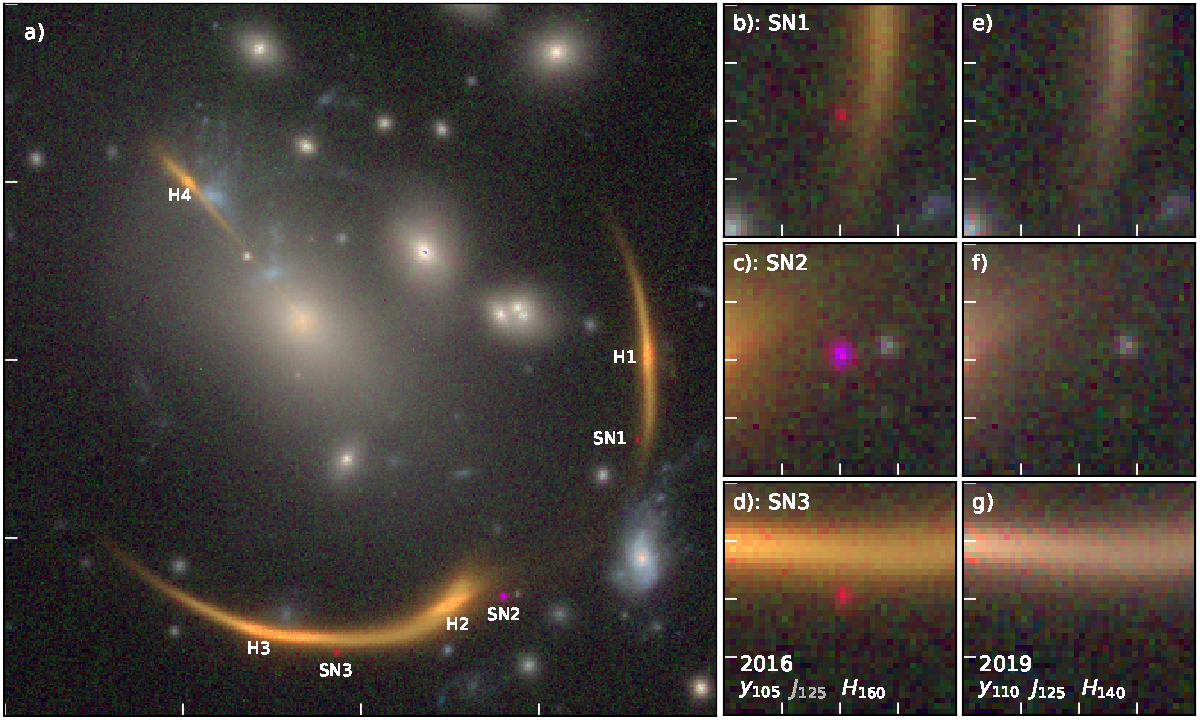
\includegraphics[width=0.9\textwidth]{Paper/Figures/fig1_layout.pdf}
    \caption{Overview of the field around the center of the MACSJ0138 cluster field and the locations of the lensed host (H1--4) and \SNABC (SN1--3) images. The wide-field view in $a)$ is 40\arcsec\ on a side with ticks indicating 10\arcsec\ intervals.  Panels b--g) show 4\arcsec\ cutouts around the lensed SN images with 1\arcsec\ ticks.  The three-color images are generated from the WFC3/IR filters as indicated; panels $b$--$d$ show the imaging from July 2016 where the SN was visible and $e$--$g$ show the later imaging from July 2019 where the the SN has faded away.  All panels use the late-epoch F125W imaging for the green channel.  Nevertheless, it is immediately clear that the SN2 image is substantially bluer than the other two, which we use in \S\ref{s:colorcurves} below to constrain the transient classification as a likely Ia supernova explosion.}
    
    \label{fig:layout}
\end{figure*}

%%%%%%%%%%%%%%%%%%%%%%%%%%%%%%%%%%%%%%%
%%%%%%  Lens model
%%%%%%%%%%%%%%%%%%%%%%%%%%%%%%%%%%%%%%%
\section{Strong Lensing Analysis}
\label{s:lensing}

\subsection{Multiple images}
\label{ss:images}

\XXX{Would an empirical estimate of the relative magnifications from the host images help?  Images 2&3 are blobbed together, but could possibly come up with a number like $\mu_1:(\mu_2 + \mu_3)$.}

\subsection{Time delay}
\label{ss:timedelay}

%%%%%%%%%%%%%%%%%%%%%%%%%%%%%%%%%%%%%%%
%%%%%%  SN Classification
%%%%%%%%%%%%%%%%%%%%%%%%%%%%%%%%%%%%%%%
\section{Transient Classification}
\label{s:classifiation}


To evaluate the age of each transient image (and therefore constrain the lensing time delay between images), it is valuable to have a firm determination of the transient's class.  The range of possible transients is broad, encompassing normal SNe, superluminous SNe \citep{galyam_luminous_2019}, fast transients \citep{berger_fast_2013, drout_rapidly_2014}, and even gravitational microlensing events \citep{rodney_two_2018,kelly_extreme_2018}.  Identifying the transient type makes it possible to use the well-developed library of spectrophotometric SN models \citep[e.g.][]{kessler_models_2019} for the time delay measurement. 
 The first-order distinction that is most important is between a Type Ia SN--understood to be the explosion of a white dwarf star in a binary system--and core collapse SN (CCSN)--the end-point of a star with mass $\gtrsim 10$M$_{\odot}$.  Given the limited data available for this transient, we will not attempt a more fine-grained classification, though in principle that could be achieved with spectroscopy and multi-band photometry upon arrival of the final image.  
 


As a first step, we can use inferences from the lens model to establish a strong prior against any of the various rapidly evolving and low-luminosity stellar transient classes.  
The expected time delays between the images are $\sim100$ observer-frame days, 
but we see that three images of the transient are visible simultaneously.
From this we can infer that the visibility time of the transient in the $z=1.95$ rest-frame must be at least $\sim$30 days. 
Similarly, with expected magnifications in the vicinity of $\mu\sim10$, the measured apparent magnitudes near 23 AB mag translate to a rest-frame absolute magnitude near $M_B \sim-19.5$ mag (too bright to be a nova, luminous blue variable, or other low-luminosity stellar transient).
Taken together, these indicators strongly suggest that the transient is a supernova (SN). 

Although we have invoked the lens model in this analysis, note that the inferences are not strongly dependent on the specific lens model predictions.  To make the observed transient images consistent with a fast or low-luminosity transient, the time delays and/or magnifications would have to be changed by more than a factor of 2.  In the analysis to follow, we will work under the assumption that the transient is a SN. 

\subsection{Host galaxy properties}
\label{ss:host}

We first seek to classify this transient {\it circumstantially}, using measured properties of the host galaxy stellar population to infer the type. Although Type Ia SNe are found in all types of galaxies, CCSNe are limited to galaxies with relatively young stellar populations.  We can therefore infer some information about the SN type using the observed host properties combined with knowledge of the relative rates of Type Ia and CCSNe in different stellar populations \citep{mannucci_rates_2005,foley_classifying_2013}.  In the case of the host galaxy MRG0138, we have very stringent limits on the star formation rate. This galaxy is a high-mass but very quiescent galaxy, with a specific star formation rate of $\sim10^{-11.3}$ yr$^{-1}$  and a stellar population that is well-matched by an exponential star formation history with an age of $1.4$ Gyr \cite{newman_resolving_2018}.  The massive stars that end as CCSN explosions have main-sequence lifetimes of $\lesssim 40$ Myr,  making it highly unlikely that MRG0138 retains any significant population of massive stars \SR{this should be revised, b/c of total mass.  Focus instead on the relative probability. as discussed on telecon}


Discussion from Newman et al. \citep{newman_resolving_2018-1}.

Conclusion: the host is a red-dead elliptical. It is most likely a Type Ia SN.

\subsection{Light curve analysis}
\label{ss:lightcurve}

\SR{TODO: describe color-mag based classification checks}
Figure~\ref{fig:colormag} shows the location of \SNABC in color-magnitude space, comparing the de-magnified apparent F160W magnitude against the observed F105W-F160W color.  

\SR{TODO: describe the interpretation of possible source-plane or lens-plane extinction}


\begin{figure*}
    \centering
    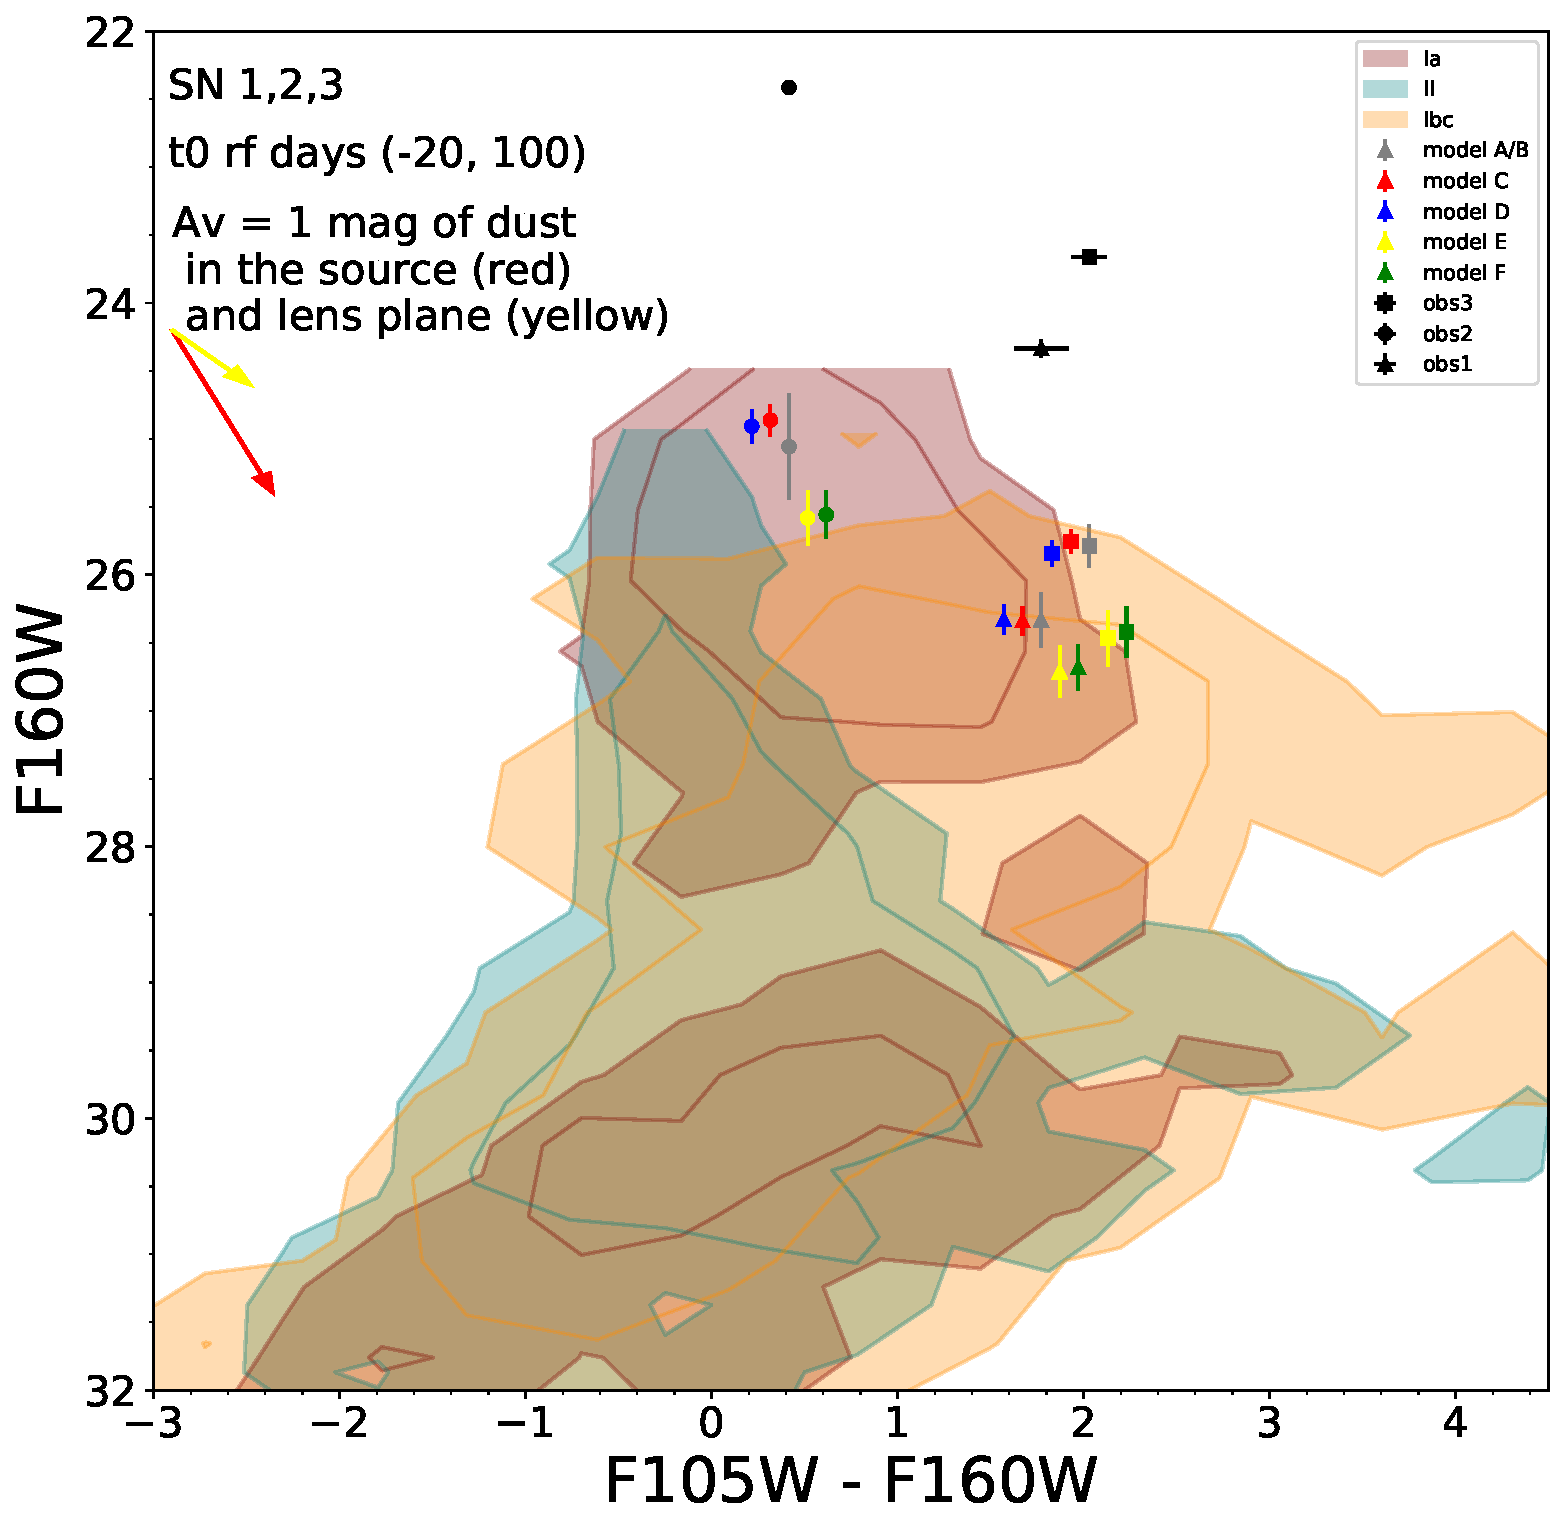
\includegraphics[width=0.45\textwidth]{Images/color_mag_contours_all.pdf}
    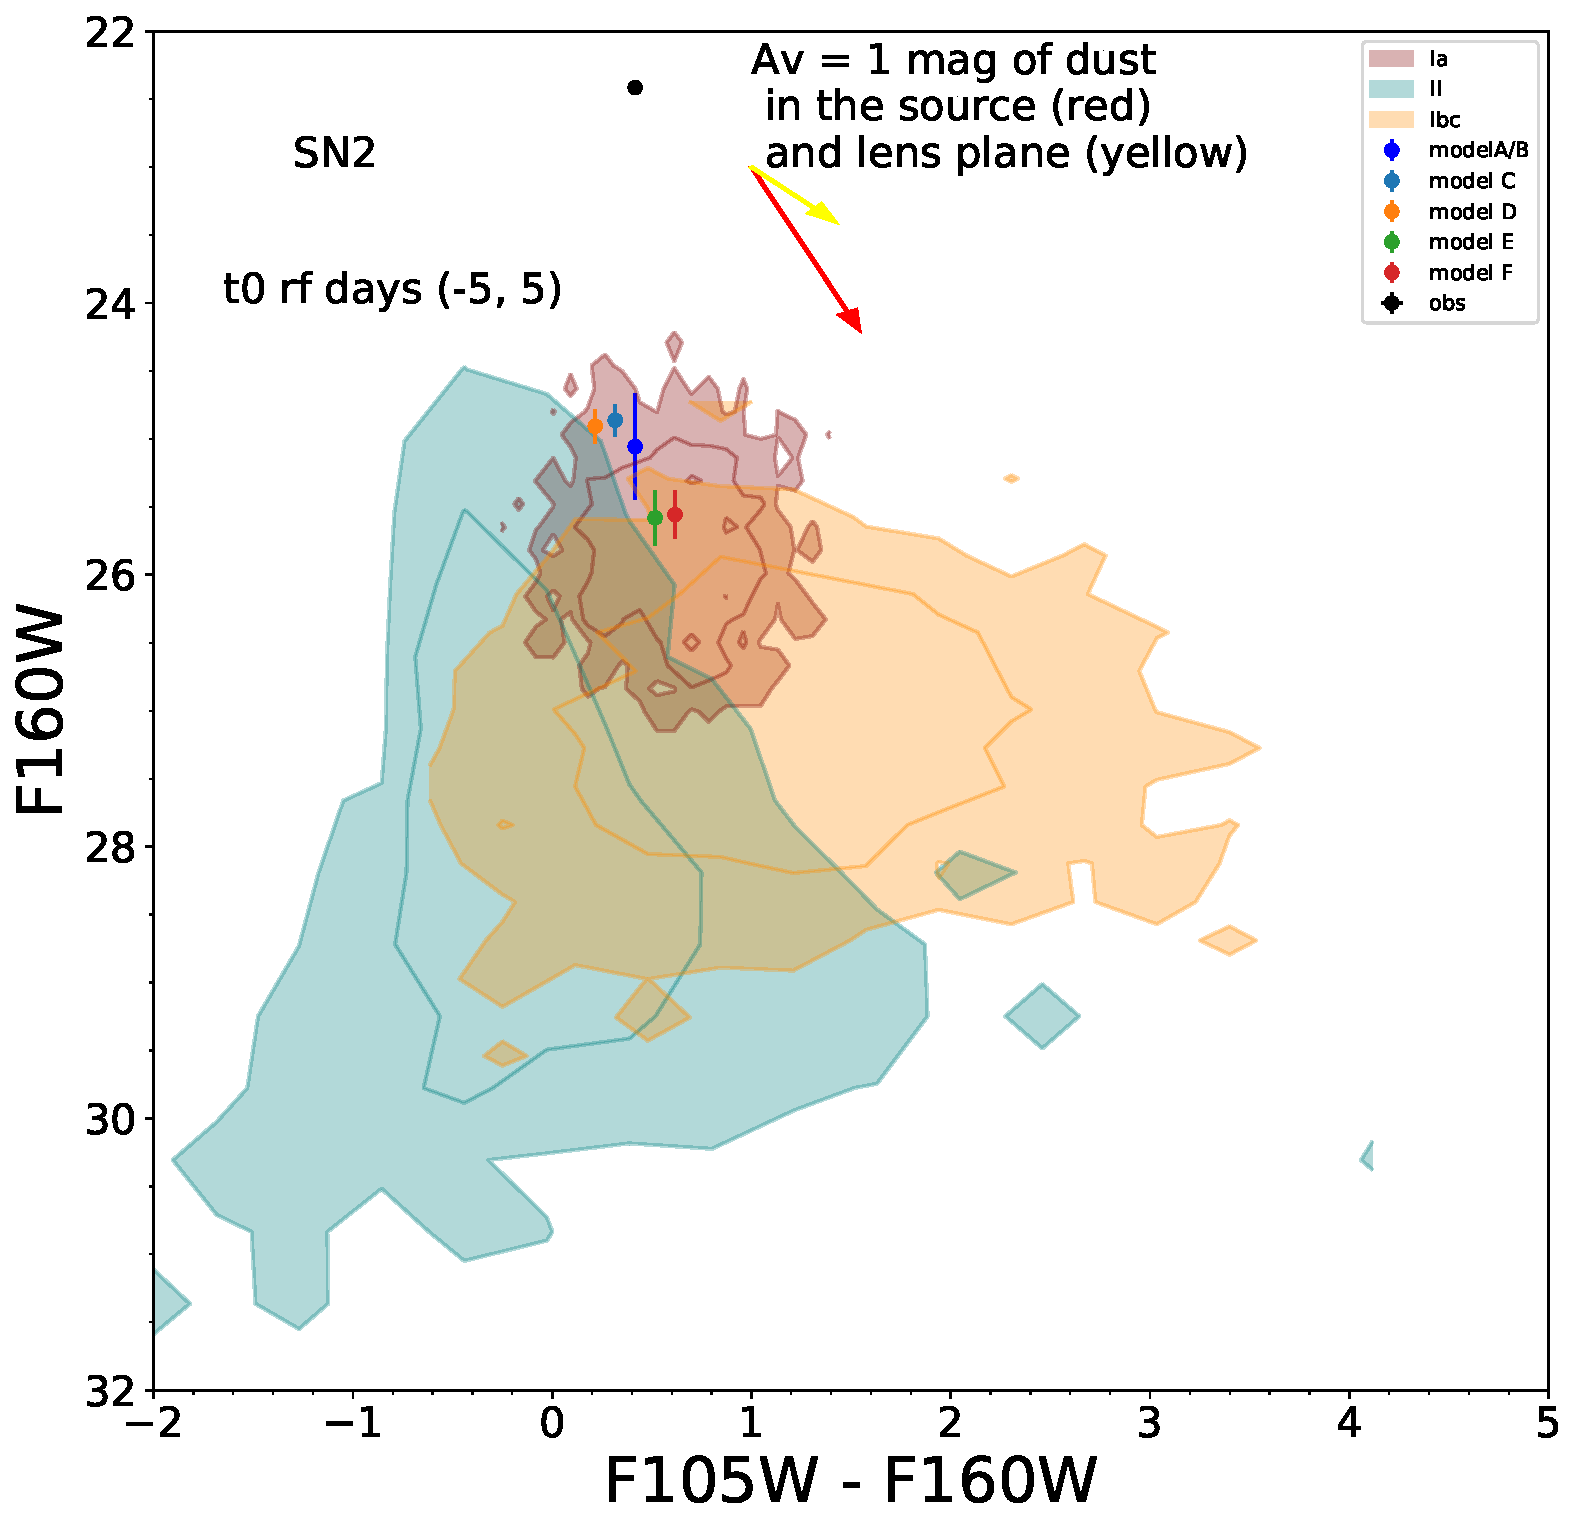
\includegraphics[width=0.45\textwidth]{Images/color_mag_contours_image2.pdf}
    \caption{Classification information for \SNABC based on its position in color-magnitude space. Contours show the population distributions for normal SNe of Type Ia (red), Type Ib/Ic (gold), and Type II (green).  These population contours are drawn to enclose 68\% (interior solid lines) and 95\% (exterior shaded regions) of each SN population.  Each SN sub-class was simulated at $z=1.95$, and samples from their expected light curves were drawn uniformly in time. 
    The left-hand plot includes time samples ranging from a rest-frame time of 20 days prior to 100 days after peak brightness. The right-hand plot limits this range to $-5<t<5$ rest-frame days.  \SR{Kyle: did the sims for these plots include some dust extinction assumption, or range of Av values? Yes they used host dust w Rv drawn normally around 3.1, sigma 0.5, then the Av assigned using your Ia and CC pAv distributions from Rodney et al 2014a; I have updated images on evernote w a lens plane dust vector but going to hold off on putting those in until I talk to you to make sure what I did made sense there}  The observed photometry from each SN image appears with a cluster of 6 points in the plot: black markers show the observed (uncorrected) color-magnitude values, and colored markers show the demagnified value---after removing the magnification values inferred from each of the five lens model variants. Colored markers are slightly offset from the observed F105W-F160W color value for clarity.   The right-hand plot shows only the photometry for image 2, which is most strongly consistent with a Type Ia SN near peak brightness.   Red vectors in each diagram show the impact that $A_V=1$ magnitude of dust extinction would have on the observed photometry of \SNABC.  
    }
    \label{fig:colormag}
\end{figure*}


%%%%%%%%%%%%%%%%%%%%%%%%%%%%%%%%%%%%%%%
%%%%%%  Time Delay Constraints
%%%%%%%%%%%%%%%%%%%%%%%%%%%%%%%%%%%%%%%
\section{SN Age and Time Delays}
\label{s:age_and_timedelays}

In this section, we constrain the relative time delays of \SNABC by using two separate methods to estimate the age of the SN at each image during the single observed epoch. The preferred method of SN time delay measurements involves measuring the time of peak brightness for the SN at each image by fitting the light curves, and taking the difference between each measurement as the relative time delay \citep[e.g.][]{pierel_turning_2019,dhawan_magnification_2019,huber_strongly_2019}. With only a single observed epoch, this method is impossible due to model parameter degeneracies, and we must rely on age constraints using color (section \ref{s:colorcurves}) and brightness (section \ref{s:lightcurves}) to estimate relative time delays. The final time delay measurements are presented in section \ref{s:timedelays}.

\begin{deluxetable*}{crrrrrrr}
    \tablecaption{\label{tab:model_evidence}Model Preferences}
    
    \tablehead{\colhead{Model} & \colhead{$\mu_1$} & \colhead{$\mu_2$} & \colhead{$\mu_3$}  &\colhead{$t_2-t_1$} & \colhead{$t_3-t_1$}& \colhead{$t_4-t_1$} & \colhead{Bayesian Evidence}}
\startdata
\textit{C} & 6.324 & 9.526 & 6.879 & 180.3 & 82.7&7402.8&$-15.18\pm0.33$ \\
\textit{D} & 6.281 & 9.923 & 7.472 & 184.4 & 85.3&7034.9&$-13.46\pm0.31$ \\
\textit{E} &8.942  & 18.48 & 13.257 & 103.6 & 50.2&5876.8&$-8.91\pm0.27$ \\
\textit{F} & 8.699 & 18.069 & 12.719 & 108.3 & 53.7&6020.5&$-9.67\pm0.28$ \\
\enddata

\end{deluxetable*}


\subsection{Color Curve Age Constraints}
\label{s:colorcurves}

The color of a Type Ia SN evolves substantially over its lifetime, as the photosphere expands and cools, revealing different layers of the expanding shell and driving episodes of recombination \citep{woosley_type_2007,kasen_type_2009}. Since the phenomenon of gravitational lensing in general is achromatic, this color evolution makes it possible to derive an age constraint that is largely independent of the lens model.  One important caveat to this principle is that {\it microlensing} effects are not generally achromatic, because the microlensing caustics may cause differential magnification on the scale of the SN radius \citep{goldstein_precise_2018,foxley-marrable_impact_2018,bonvin_impact_2019}.  Hence, if the expanding SN shell has a color gradient then microlensing may introduce spurious features in the observed colors of the SN \SR{citations: vernardos, kochanek, etc}.   Goldstein et al. \cite{goldstein_precise_2018} found that such chromatic microlensing is most likely not present for lensed Type Ia SNe in the period up to about 25 rest-frame days after explosion ($\sim$15 observer days after peak brightness for \SNABC). Only image 2 is likely in the achromatic microlensing phase, but Goldstein et al. \cite{goldstein_precise_2018} found extremely small deviations in the rest-frame $U-V$ color curve due to microlensing at the 68\% confidence interval, and up to a $\sim0.2-0.4$ mag difference with 99\% confidence. While such extreme microlensing could alter the results for images 1 and 3, it would not alter the measurement of image 2 as it is likely in the achromatic phase.

We use version 2 of the SuperNova Time Delays (SNTD) package\footnote{Link to version 2} both in this section and section \ref{s:lightcurves}, which has several improvements over the original SNTD package \citep{pierel_turning_2019}. The SNTD package employs a nested sampling algorithm within three separate methods to measure time delays, and is designed to fully utilize the information present in SN light curve templates \citep[e.g.][]{hsiao_k_2007,kessler_results_2010,pierel_extending_2018} to reduce the impacts of microlensing and make more accurate measurements. 

We first obtain a constraint on the time delay from the SN color (F110W-F160W) at each image, which is completely independent from the lens model and relatively insensitive to microlensing. We use the "color" method present in SNTD, which attempts to reconstruct the intrinsic color curve using the SALT2 model as a template \citep{guy_salt2:_2007}. This method fits the age of each image simultaneously, while also varying the SN model parameters. Joint and marginalized posterior distributions
from SNTD for SALT2 parameters and measured ages for each image are shown in the appendix. The result of this process is seen in figure \ref{fig:colorcurve2} for image 2 (and in the appendix for images 1 and 3).  As the measured colors intersect the model at two distinct locations there are two plausible ages for image 2 of \SNABC, causing a double peaked posterior distribution. This is caused by a model parameter degeneracy that could be broken if a sufficiently precise light curve of image 4 is obtained in the future (see section \ref{s:discussion} and the appendix).



\begin{figure}
    \centering
    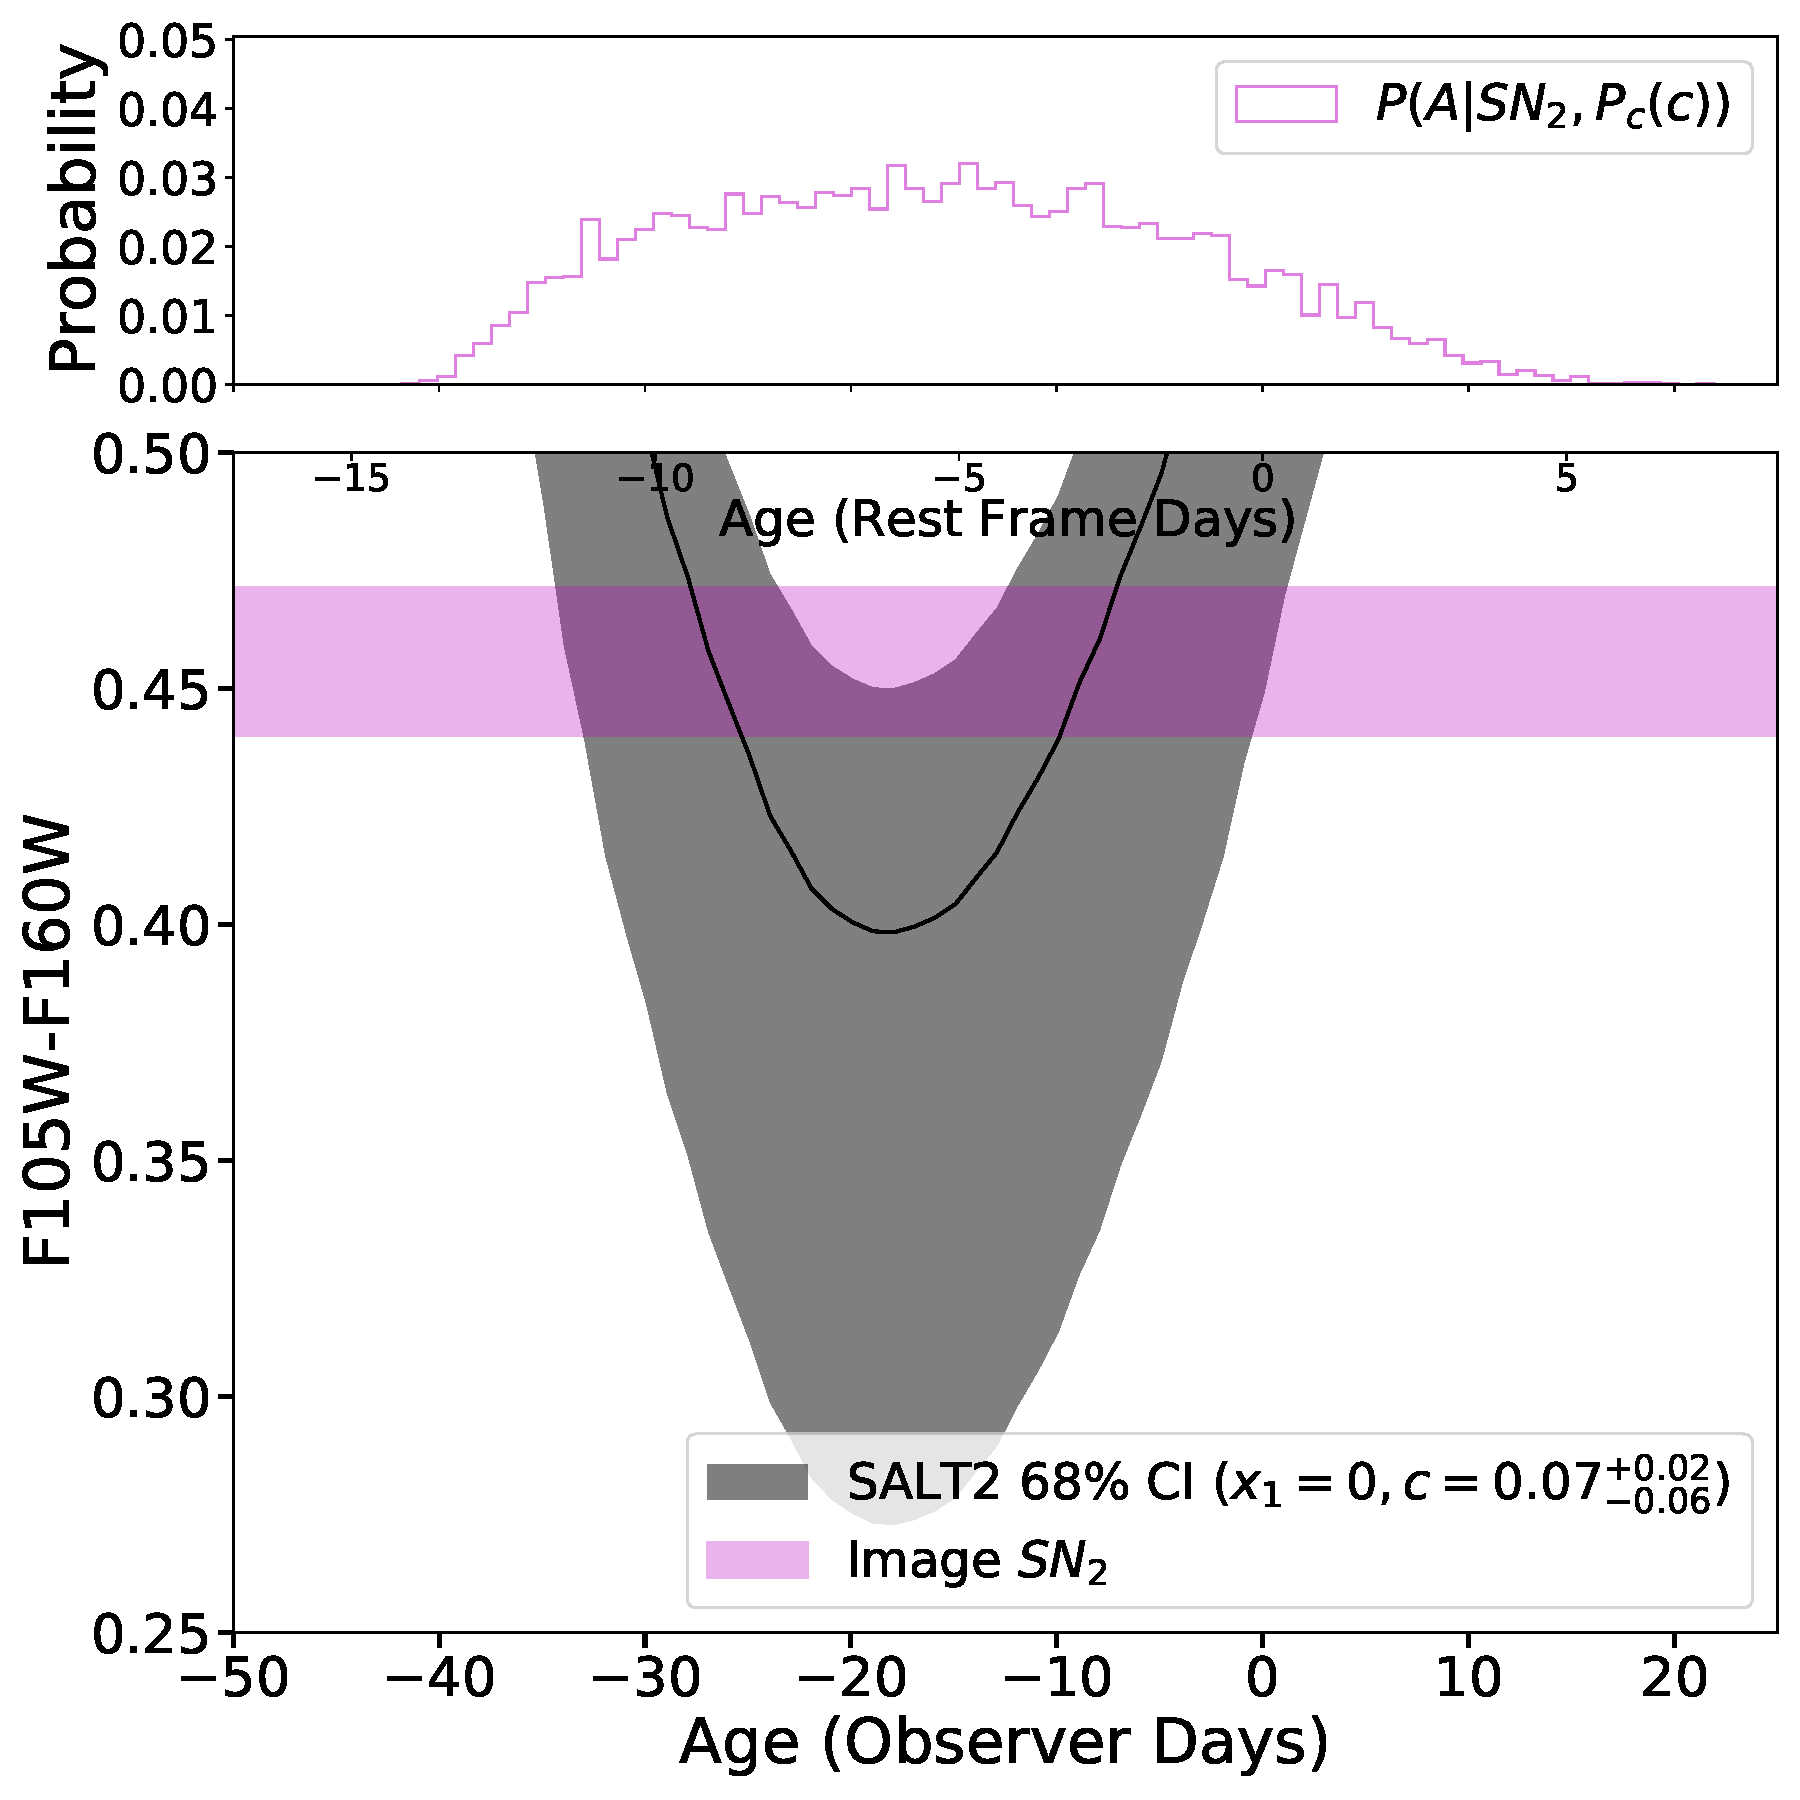
\includegraphics[width=0.45\textwidth]{Images/colorcurve_image2.pdf}
    \caption{Color-based age constraints for \SNABC image 2, using the methodology outlined in section \ref{s:colorcurves}. The upper panel shows the posterior for the age of image 2 from SNTD, using a prior on the SALT2 color parameter (c) based on known population characteristics of SNIa. The effect of adding this prior is slight, with no significant deviation from the best-fit value of c ($0.02\pm0.05$). The grey shaded region covers the 68\% confidence interval of the best-fit SALT2 color curve, with the median model shown as a solid line. The magenta shaded region shows the 1$\sigma$ range of the measured F105W-F160W color, which corresponds to a $U-V$ color in the rest-frame.}
    \label{fig:colorcurve2}
\end{figure}


\subsection{Light Curve Age Constraints}
\label{s:lightcurves}

To help break the age degeneracies in the color-based constraints, we need to use some information about the relative brightnesses of the \SNABC images.  For this step we can no longer be independent of the lens models, as we must use the lens-model-predicted magnification values to de-amplify the observed magnitudes for comparison to SN models. We expect future improvements of the lens model will further improve the constraints outlined in this section. 

For the four lens models described in section \ref{s:lensing}, we correct the observed magnitude of each image using the predicted lensing magnification ($\mu$). Next we employ SNTD's "series" method, as it is most effective for sparse sampling, to attempt a reconstruction of the intrinsic SN light curve \citep{pierel_turning_2019}. Once again the age of each image is constrained simultaneously, while also varying the SN model parameters (see the appendix for joint and marginalized posterior distributions). At this stage we adopt priors on the intrinsic SNIa luminosity \citep{rodney_type_2014} and SNIa color \citep{mosher_cosmological_2014} to help break degeneracies in the light curve model, and obtain a second constraint on the age of each SN image (Figure \ref{fig:lightcurve2}, and see the appendix for images 1 \& 3). 

After repeating this process for each of the four lens models, we use the Bayesian Evidence to determine a preferred lens model (Table \ref{tab:model_evidence}). We find significant preference for models E and F over models C and D (at $\gtrsim15\sigma$), and some preference for model E over model F (at $\sim2.8\sigma$). We therefore adopt model E as our preferred model, and use the model E light curve constraints to obtain joint posterior distributions with the lens-independent result from section \ref{s:colorcurves} (Figure \ref{fig:lightcurve2}). 


\begin{figure}[h!]
    \centering
    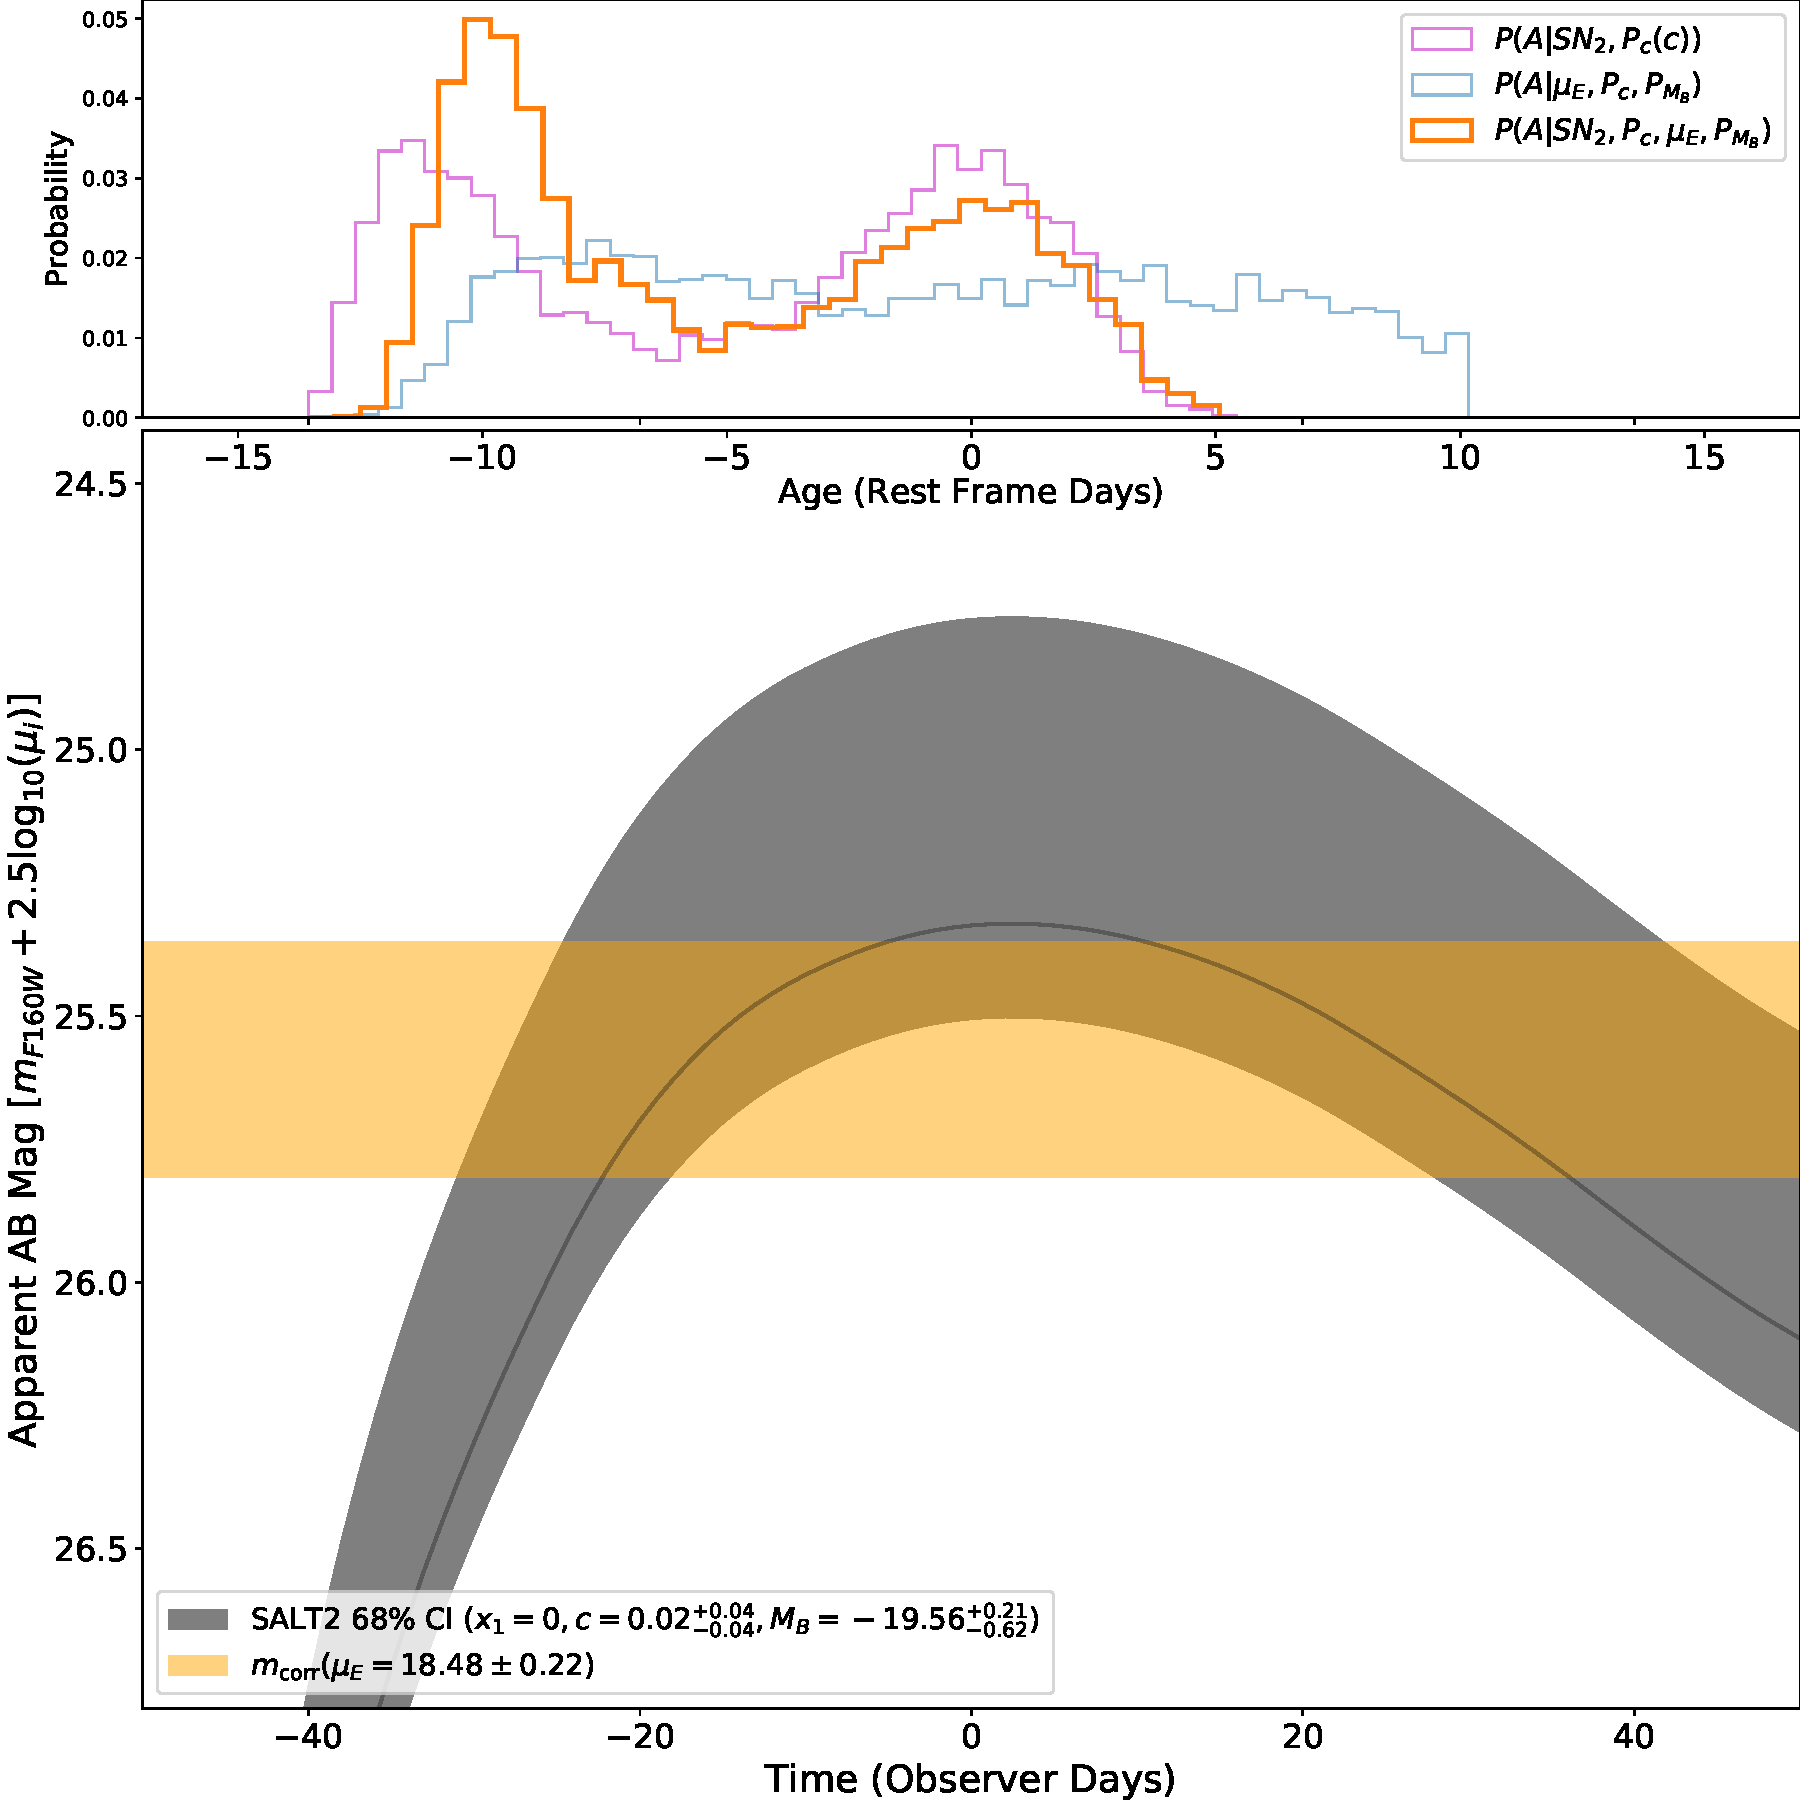
\includegraphics[width=0.45\textwidth]{Images/lightcurve_image2.pdf}
    \caption{Light-curve-based age constraints for \SNABC image 2, using the methodology outlined in section \ref{s:lightcurves}. The upper panel shows the posterior distributions from SNTD for the age of image 2 from section \ref{s:colorcurves} (magenta), section \ref{s:lightcurves} (light blue), and the combination of both methods (orange). The grey shaded region covers the 68\% confidence interval of the best-fit SALT2 light curve, with the median model shown as a solid line. The orange shaded region shows the 1$\sigma$ range of the measured (lens-model-corrected, see table \ref{tab:time_delays}) F160W magnitude, which corresponds to a V band magnitude in the rest-frame. }
    \label{fig:lightcurve2}
\end{figure}


\begin{deluxetable*}{crrrrr}
    \tablecaption{\label{tab:time_delays}Time Delays \JP{check/fix these uncertainties.}}
    
    \tablehead{\colhead{Image} & \colhead{$\mu_E$} &\colhead{$F110W_\rm{corr}$}  & \colhead{$F160W_\rm{corr}$} &  \colhead{Age}&\colhead{$t_i-t_2$}}
\startdata
\textit{1} & $8.94\pm1.61$  & $ 28.48\pm 0.24$&$26.71\pm 0.21$ &$79.10^{+45.56}_{-11.76}$&$91.31^{+62.49}_{-23.36}$ \\
\textit{2} & $18.48\pm3.78$ &  $26.00\pm0.22$&$25.58\pm0.22$ &$-16.67^{+19.14}_{13.10}$&-- \ \ \ \ \ \ \ \ \  \\
\textit{3} &$13.26\pm2.71$  &  $28.50\pm 0.24$&$26.46 \pm0.23$ &$80.46^{+20.10}_{-9.84}$&$92.60^{+37.28}_{-21.76}$ \\
\enddata

\end{deluxetable*}

\subsection{Inferred Time Delays}
\label{s:timedelays}
As discussed at the end of section \ref{s:lightcurves}, our final age constraints for each SN image are a joint posterior between the parameter estimates from sections \ref{s:colorcurves} and \ref{s:lightcurves} (see appendix for final joint and marginalized posteriors). We use image 2 as the reference image because of its likely insensitivity to chromatic microlensing,  resulting in the final time delays and uncertainties reported in table \ref{tab:time_delays}. These constraints represent an upper limit on the age (and therefore time delay) uncertainties, but they would still deliver an uncertainty of $\sim0.3\%$ on the $\sim6000$ day time delay expected by lens model E (Table \ref{tab:model_evidence}). While already dwarfed by the expected lens model uncertainty, constraints on the intrinsic SN light curve parameters gained from the future fourth image of \SNABC could improve this even further. The final posterior distribution for image 2 is bi-modal due to a degeneracy that cannot be broken by single epoch photometry, corresponding to a double-peaked intrinsic luminosity posterior for \SNABC (see appendix). If this degeneracy can be broken with the exquisite photometry expected for the final image of \SNABC, then the expected age of image 2 becomes $-31.51^{+2.23}_{-2.01}$, producing a time delay uncertainty for image 4 of $\sim0.04\%$.


%%%%%%%%%%%%%%%%%%%%%%%%%%%%%%%%%%%%%%%
%%%%%%  Discussion & Conclusions
%%%%%%%%%%%%%%%%%%%%%%%%%%%%%%%%%%%%%%%
\section{Discussion}
\label{s:discussion}


\begin{figure}
    \centering
    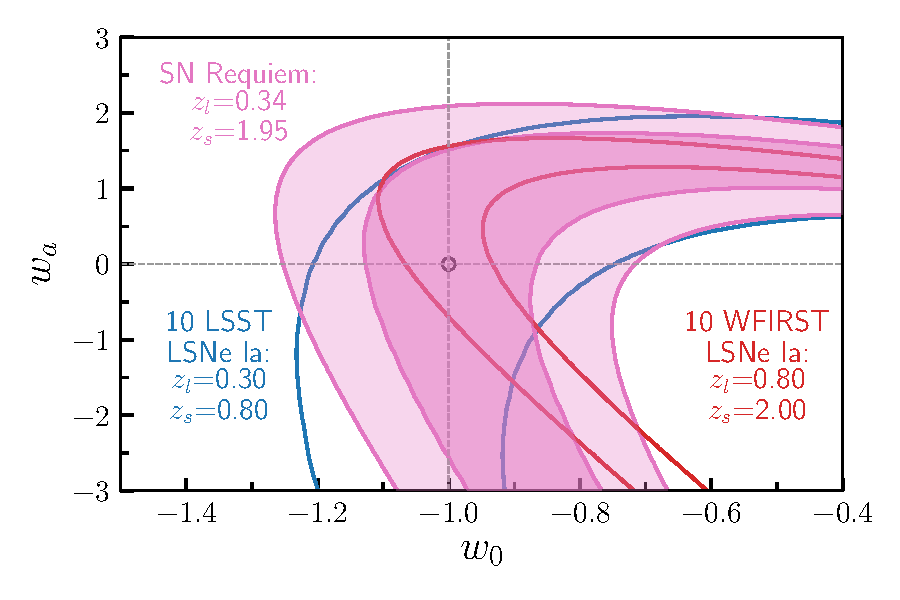
\includegraphics[width=0.5\textwidth]{Paper/Figures/snrequiem_w0wa_compared_to_lsst_wfirst.pdf}
    \caption{The unusual sensitivity of SN Requiem to dark energy equation of state parameters ($w_0, w_a$). Contours show the 1$\sigma$ confidence region for a typical sample of lensed SN time delays from LSST (blue) and WFIRST (red) compared to SN Requiem (magenta). Dashed lines and the white marker show the input values of $w_0=-1$, $w_a=0$ that were used for this simulation. In order to isolate the $w_0, w_a$ dependence, all contours are constructed assuming perfect knowledge of $H_0$, $\Omega_{m,0}$ and $\Omega_{\rm de,0}$.  SN Requiem could be highly complementary to the LSST+WFIRST lensed SN sample, due to its unusual combination of a relatively low-redshift lens ($z=0.338$) and high-redshift source ($z=1.95$). \SR{TBD: make the contours actually reflect realistic confidence regions for LSST, WFIRST and SN Requiem}. }
    \label{fig:my_label}
\end{figure}


%%%%%%%%%%%%%%%%%%%%%%%%%%%%%%%%%%%%%%%
%%%%%%  End things
%%%%%%%%%%%%%%%%%%%%%%%%%%%%%%%%%%%%%%%
\acknowledgments
Software acknowledgements: astropy, scipy, matplotlib, sep, astroquery, shapely

The Cosmic Dawn Center (DAWN) is funded by the Danish National Research Foundation under grant No. 140. 


\pagebreak


\bibliographystyle{naturemag}

\bibliography{Paper/references}

\pagebreak

\appendix

\begin{figure*}
    \centering
    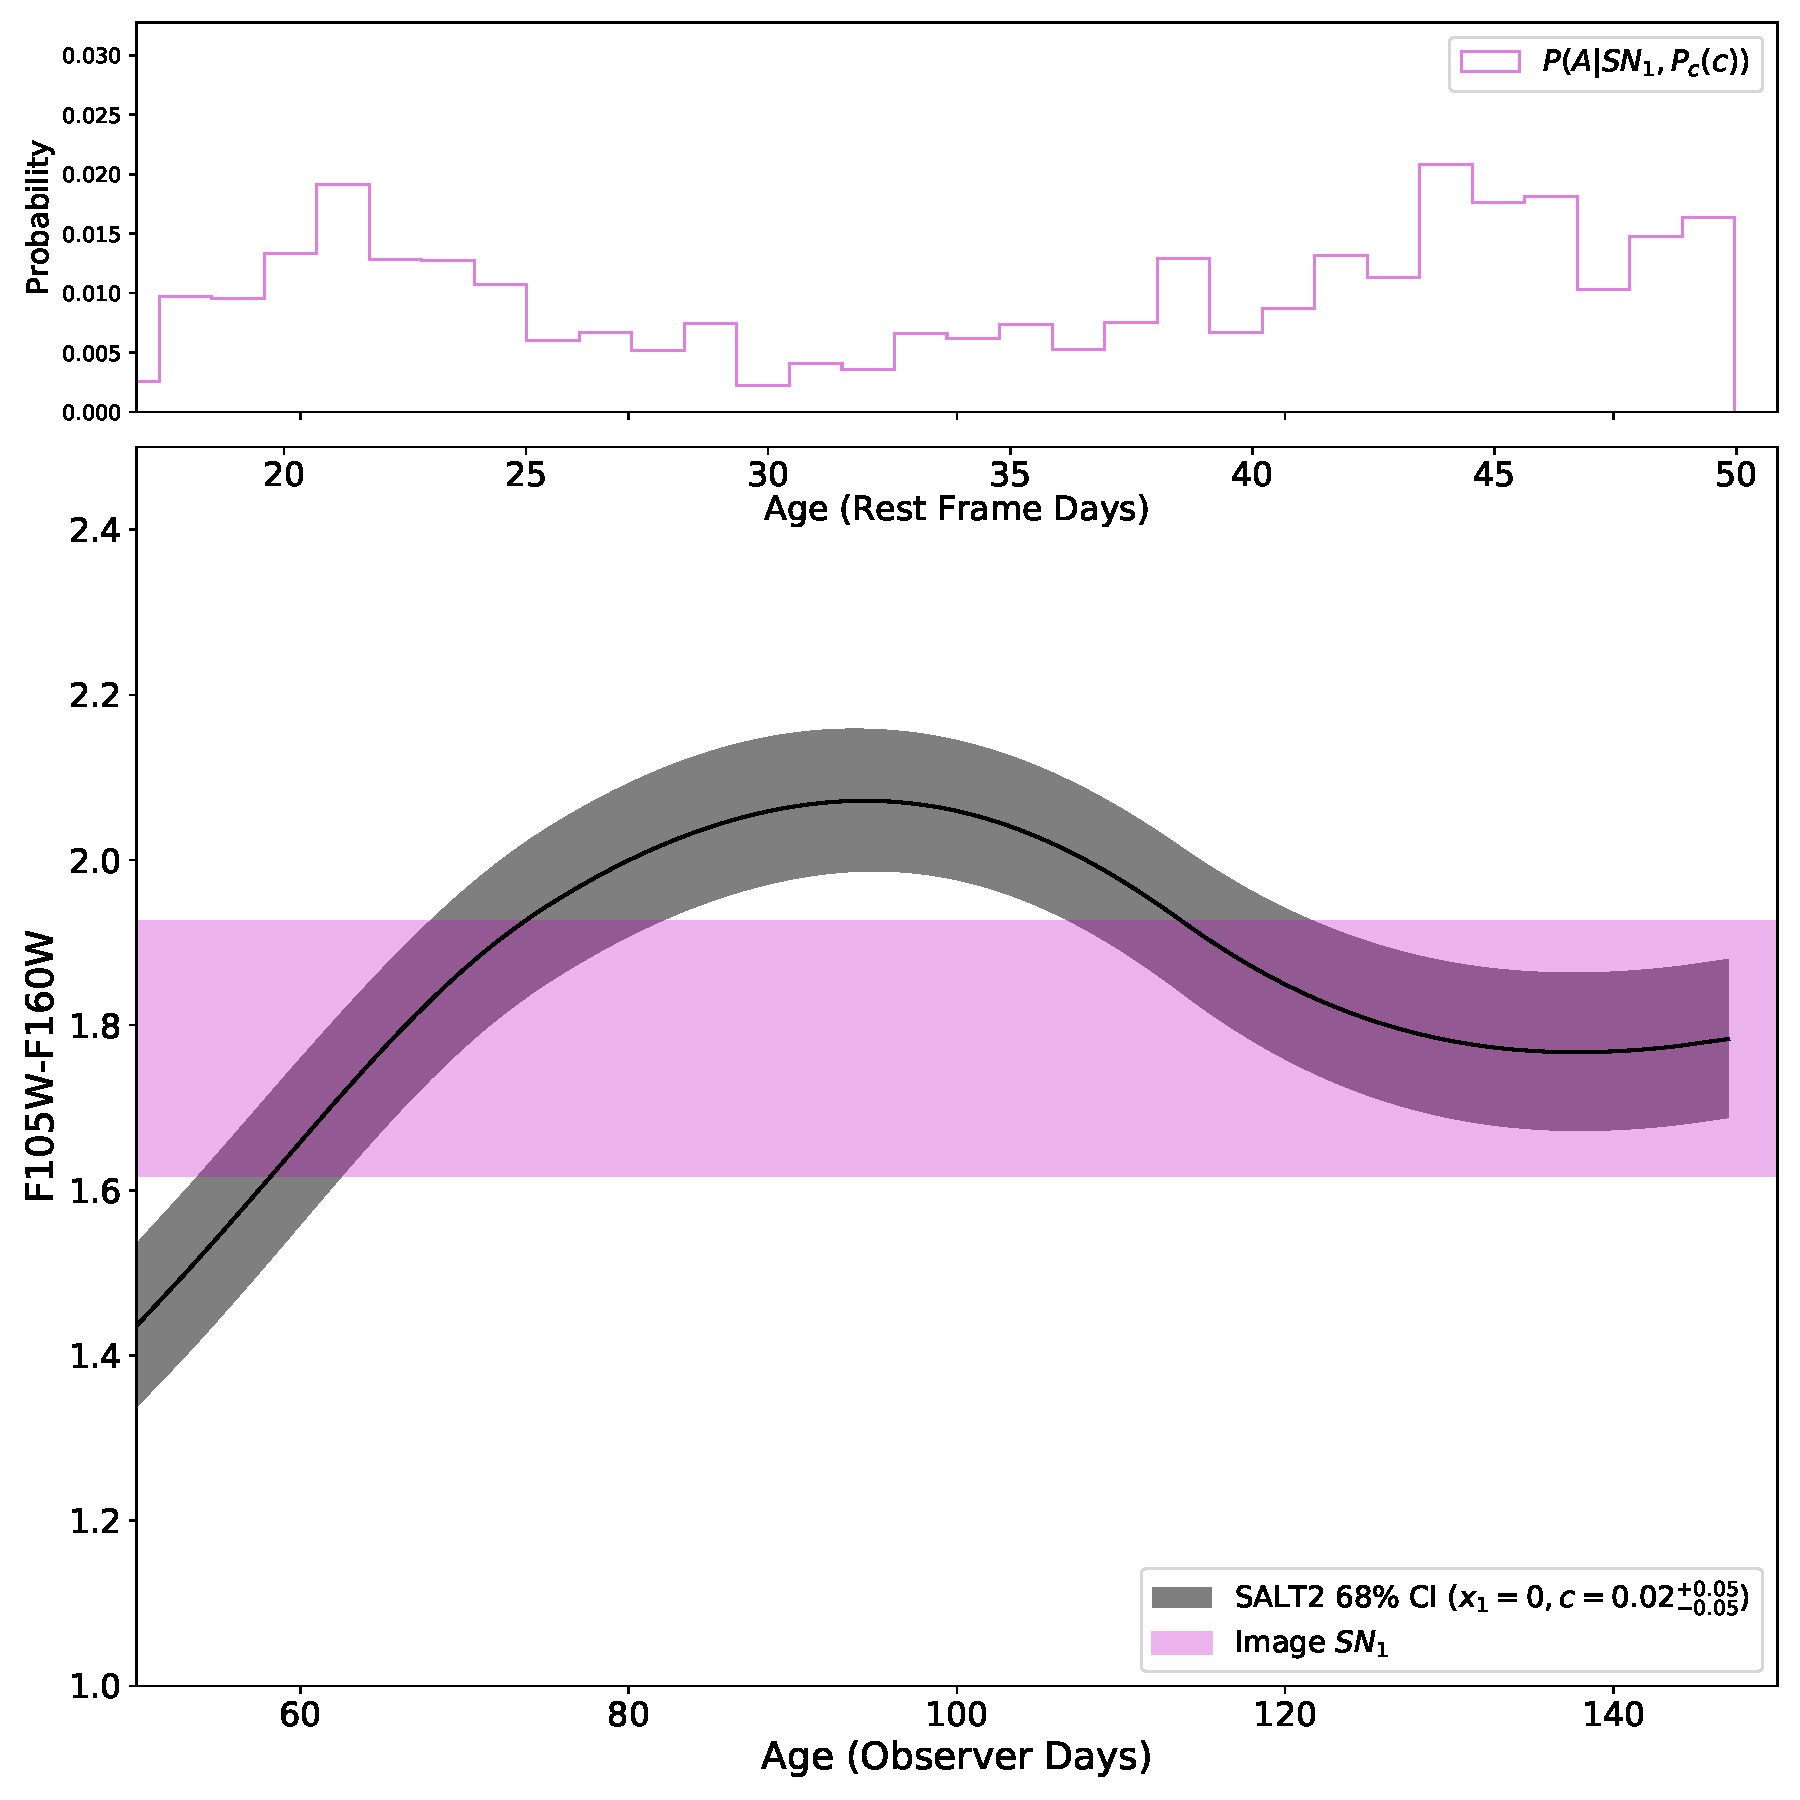
\includegraphics[width=0.45\textwidth]{Images/colorcurve_image1.pdf}
    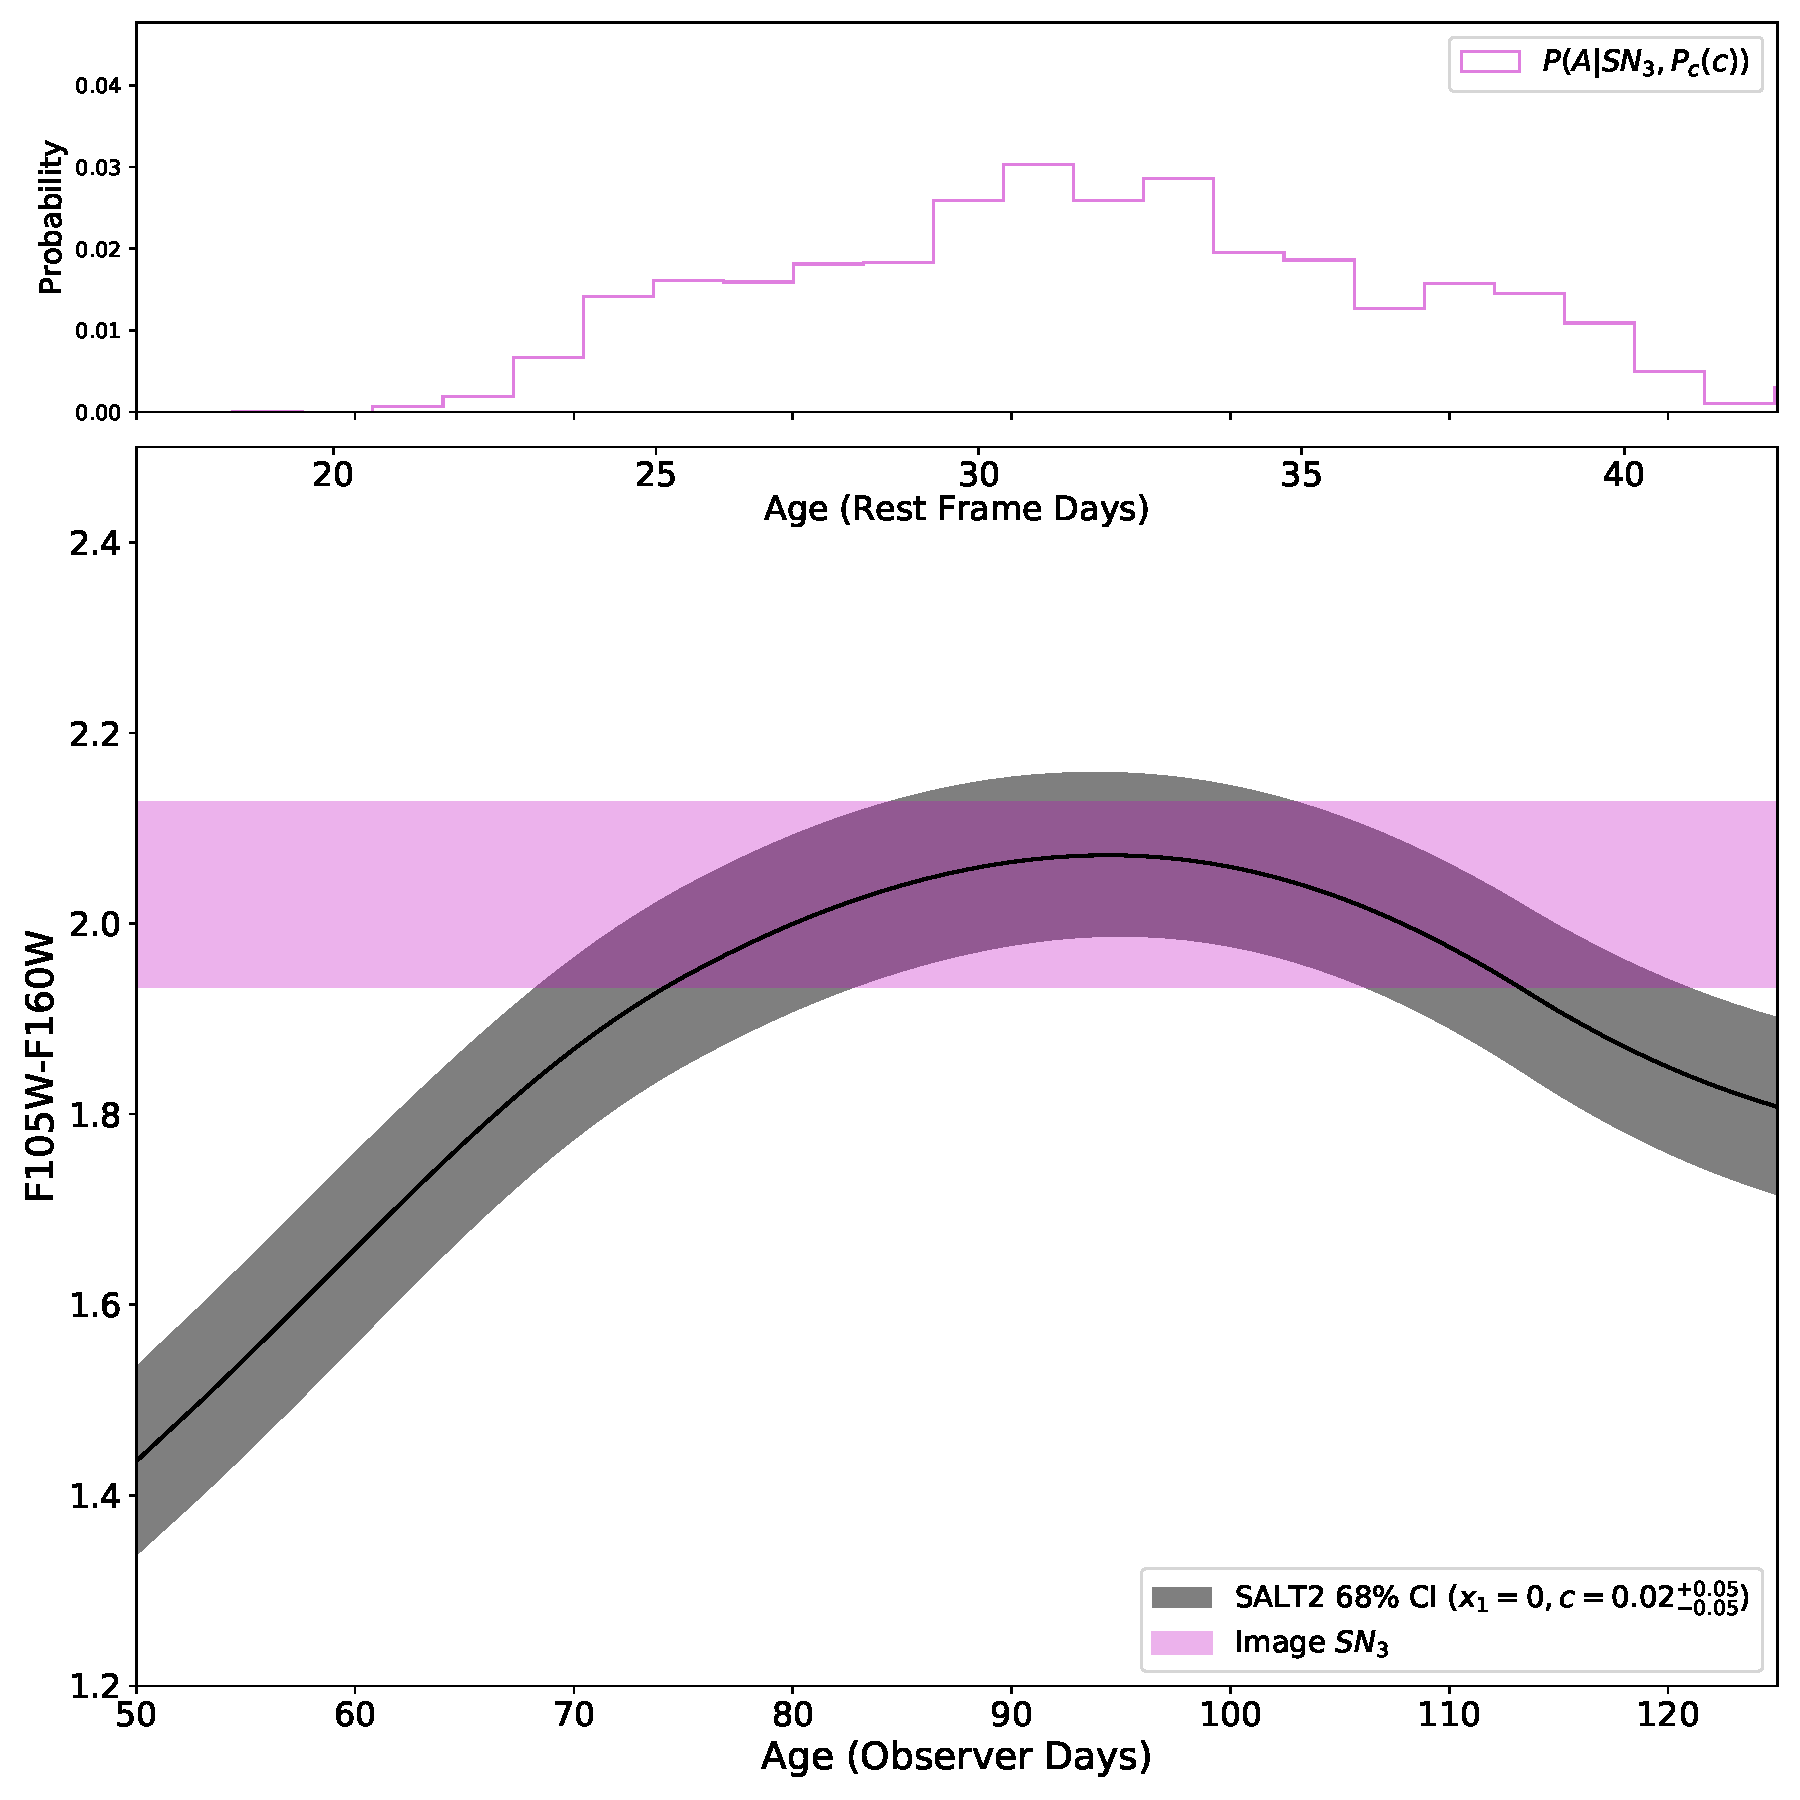
\includegraphics[width=0.45\textwidth]{Images/colorcurve_image3.pdf}
    \caption{Color-based age constraints for \SNABC image 1 and image 3, as in Fig~\ref{fig:colorcurve2}.}
    \label{fig:colorcurve13}
\end{figure*}

\begin{figure*}
    \centering
    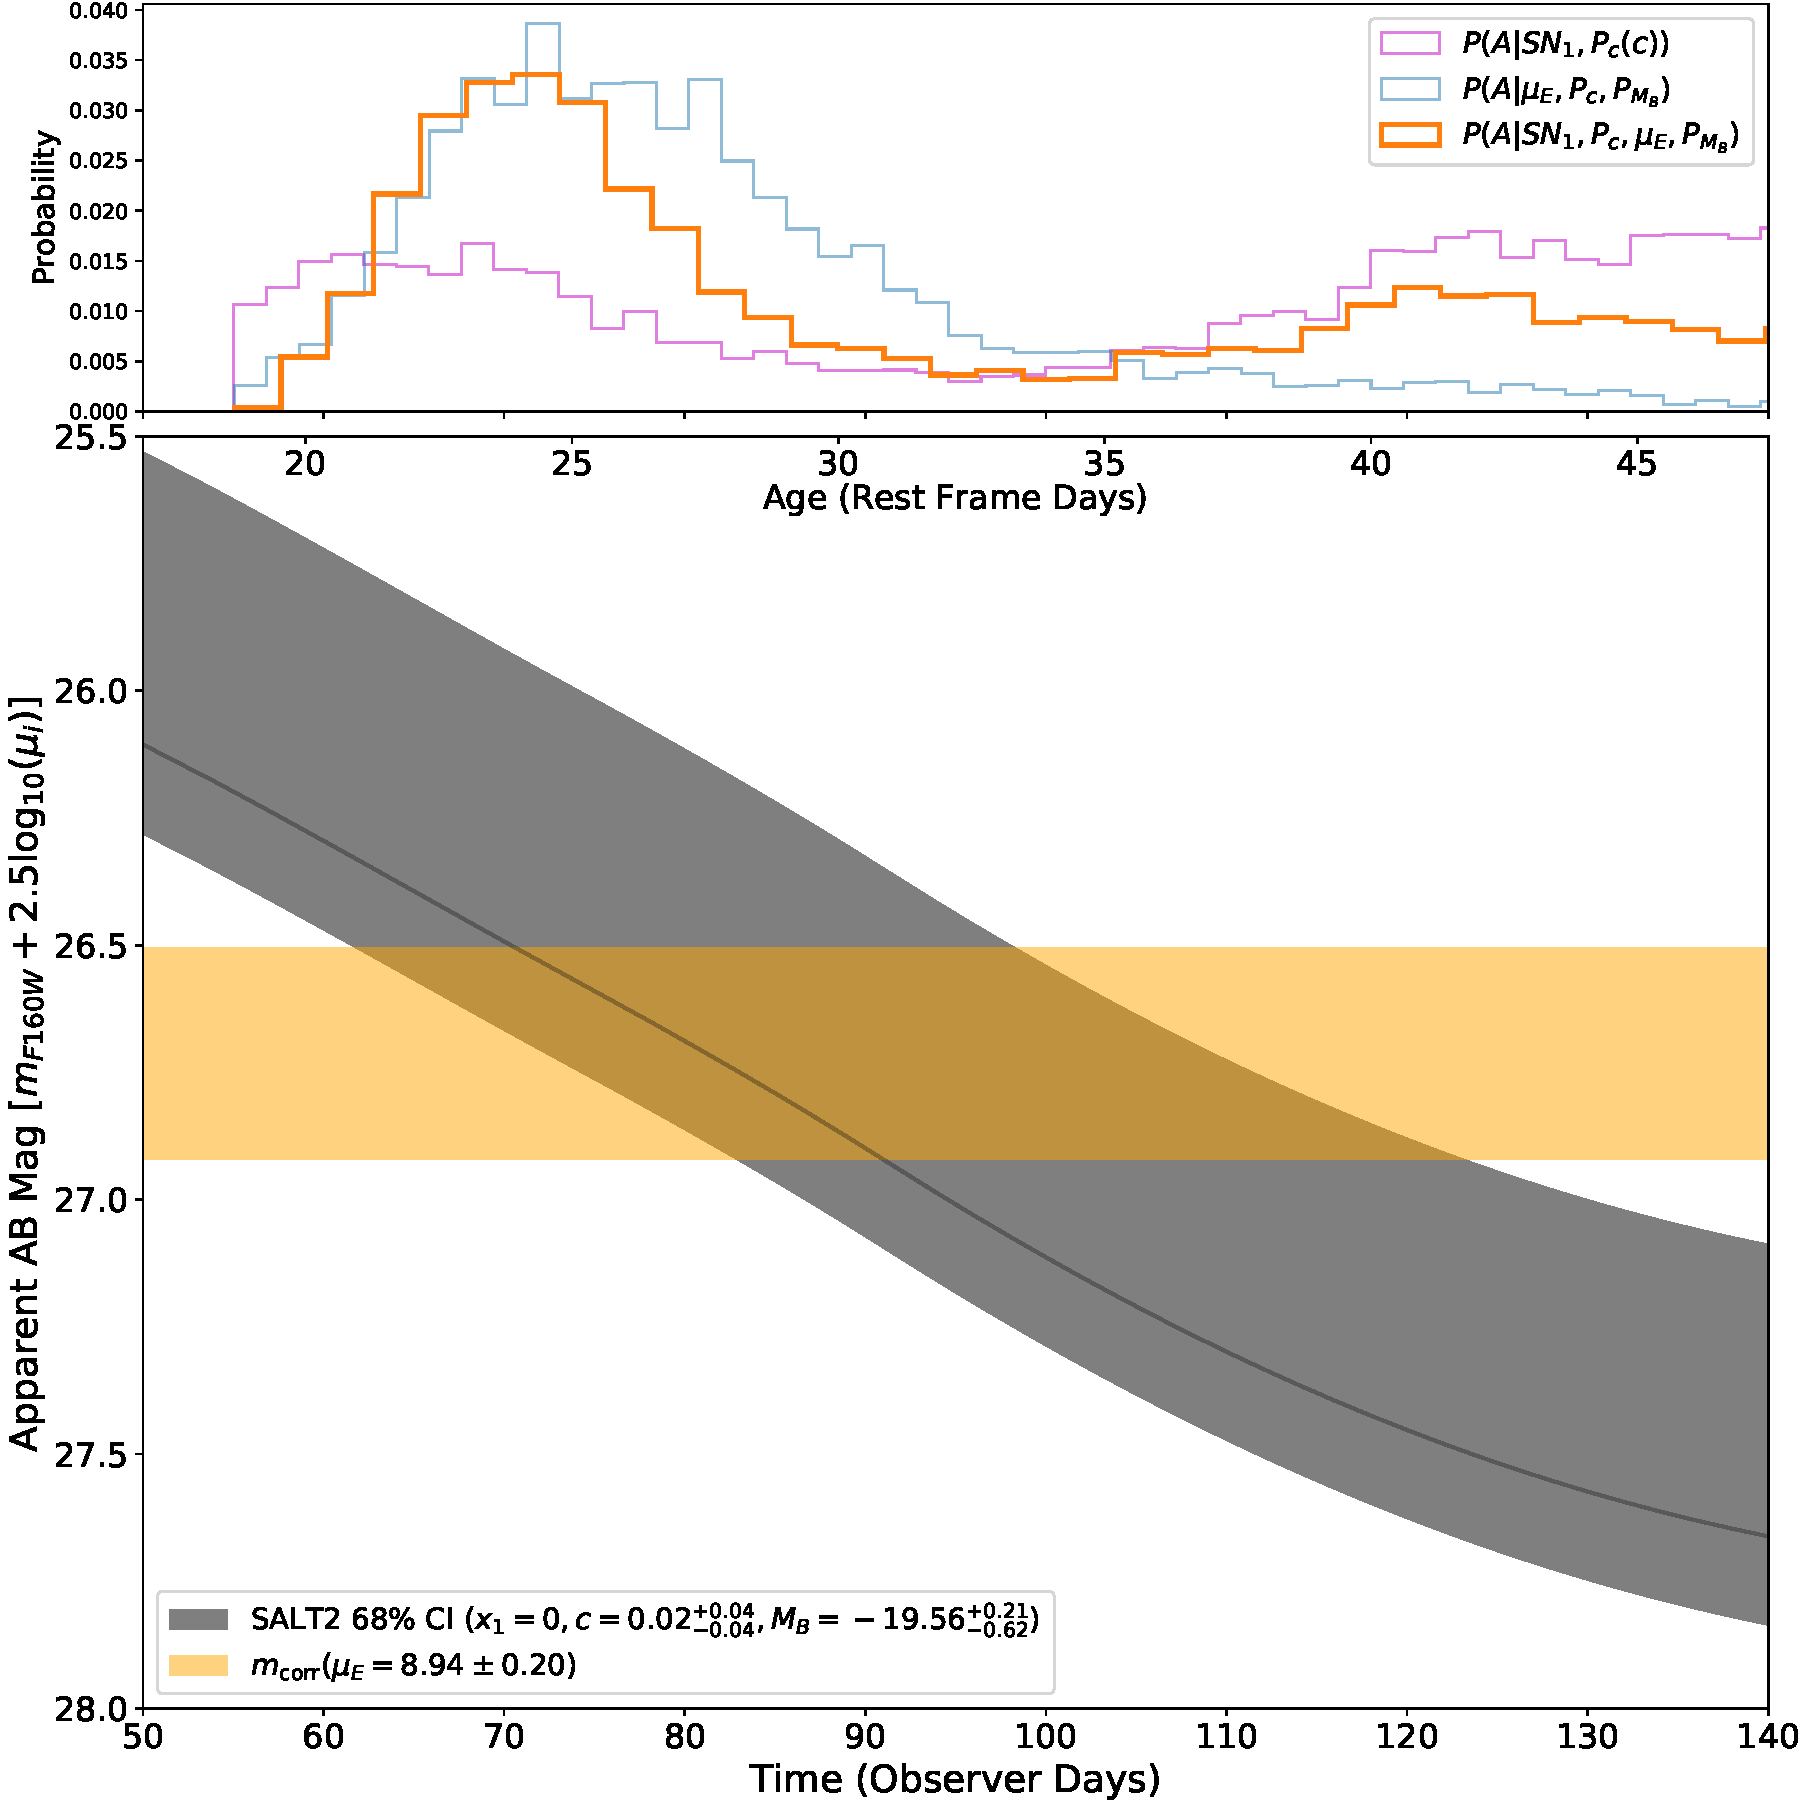
\includegraphics[width=0.45\textwidth]{Images/lightcurve_image1.pdf}
    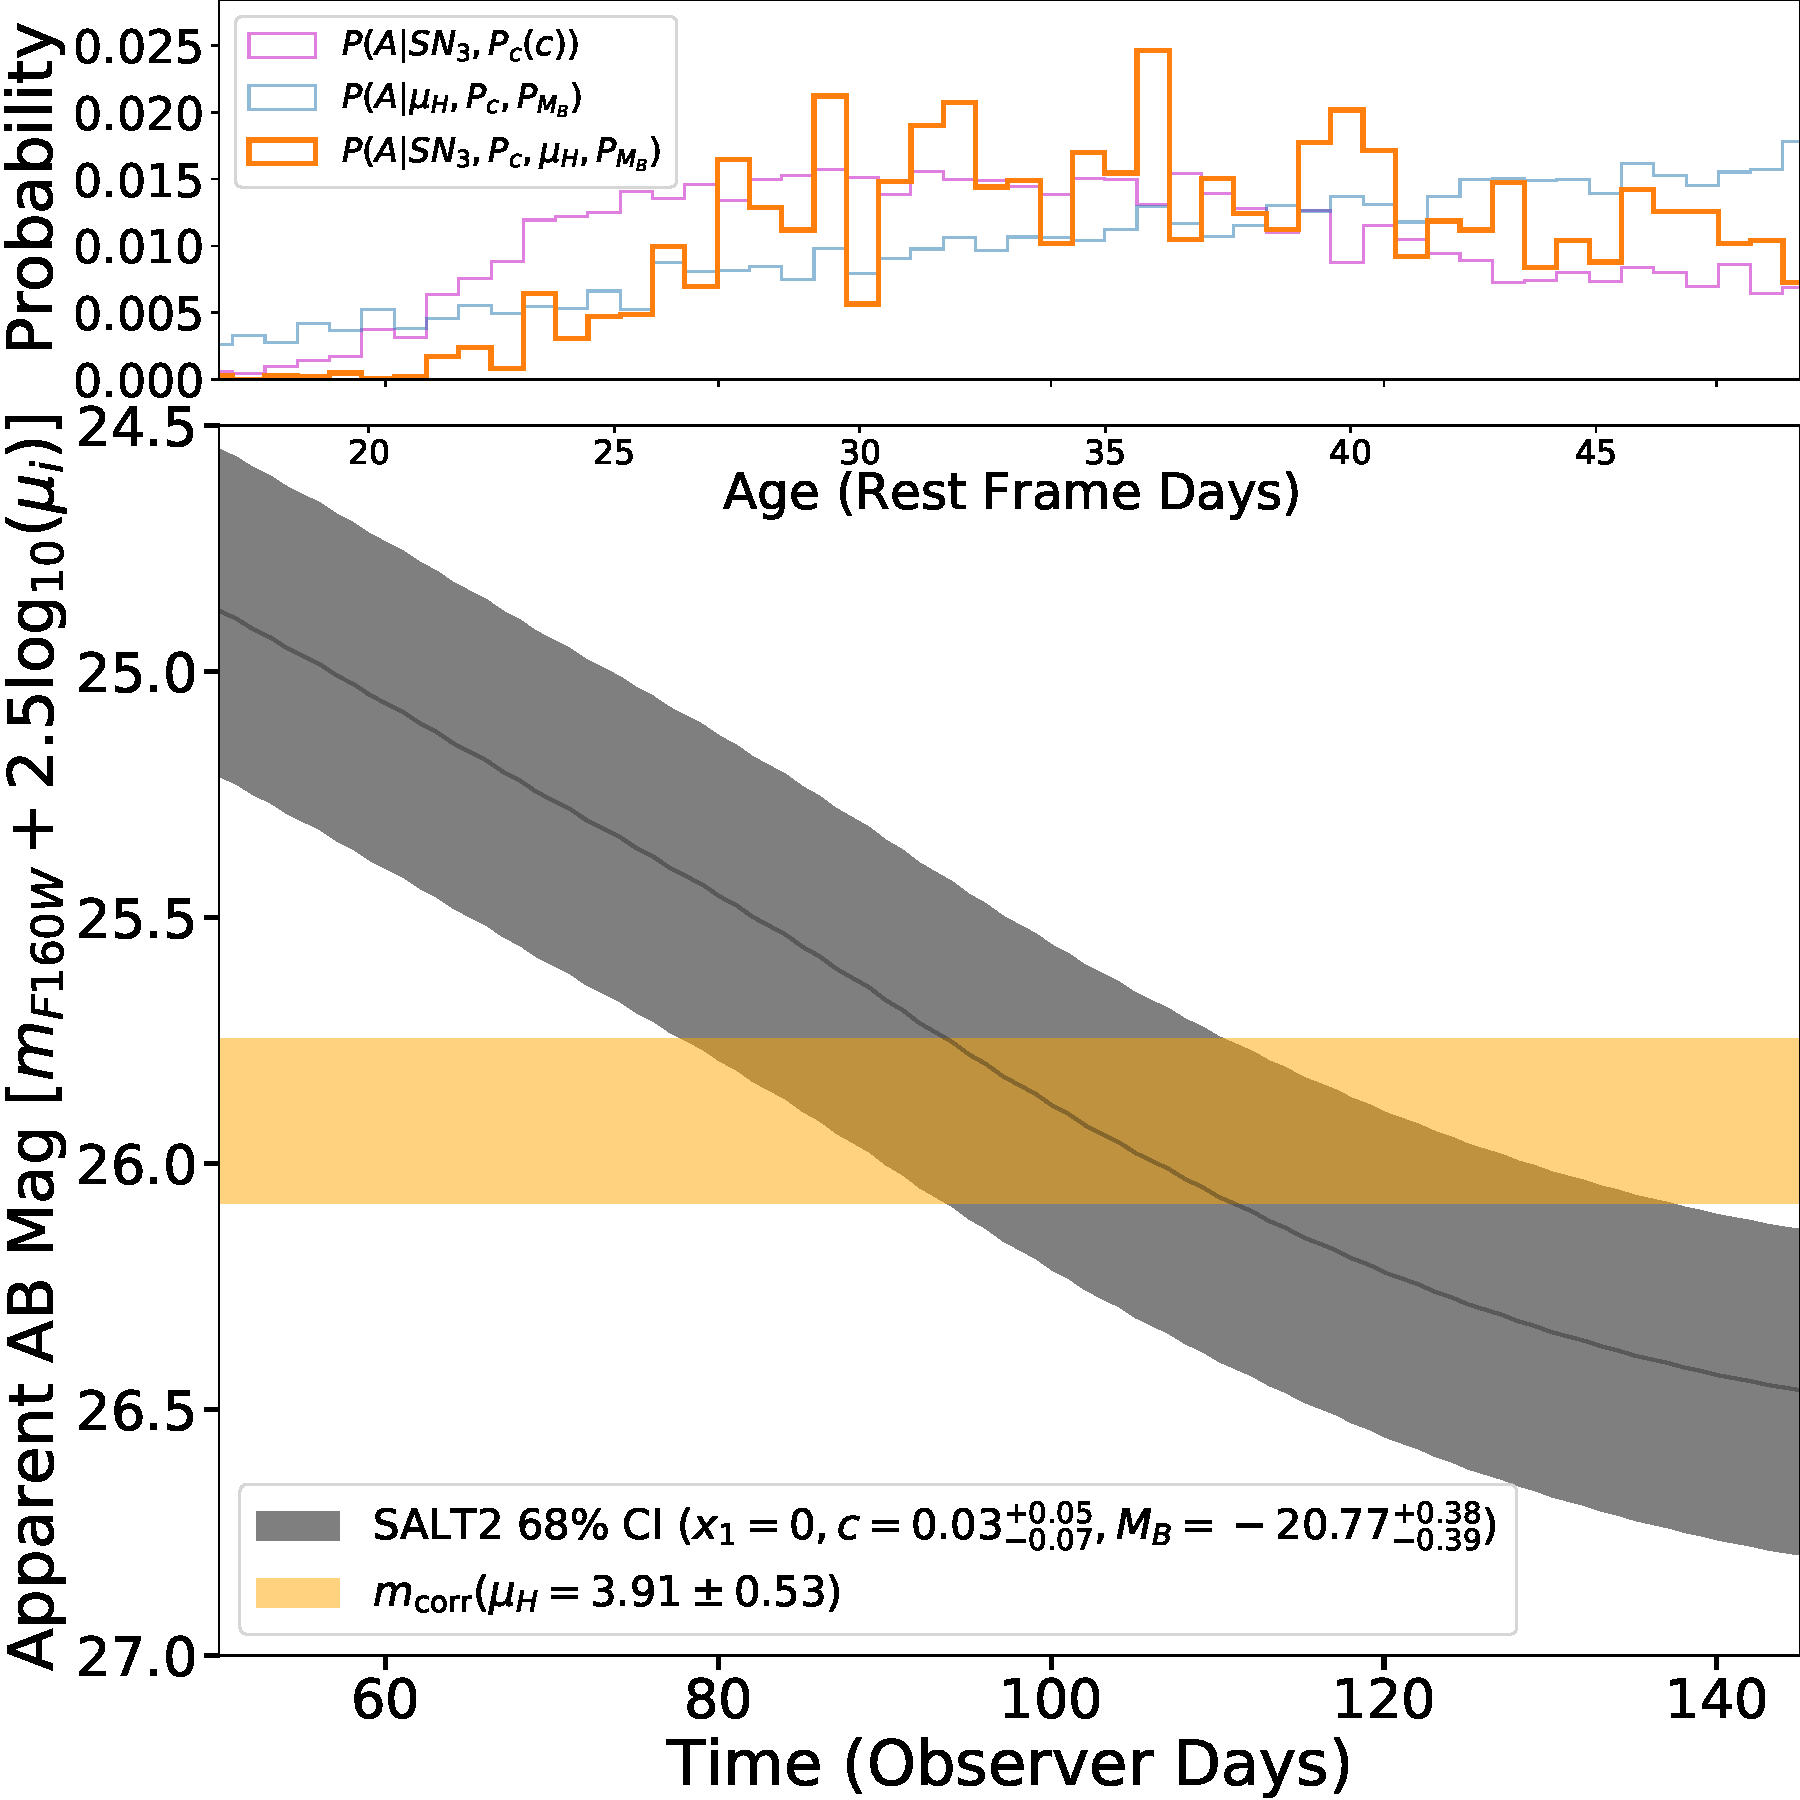
\includegraphics[width=0.45\textwidth]{Images/lightcurve_image3.pdf}
    \caption{Light-curve-based age constraints for \SNABC images 1 and 3.}
    \label{fig:lightcurve13}
\end{figure*}

\begin{figure*}
    \centering
    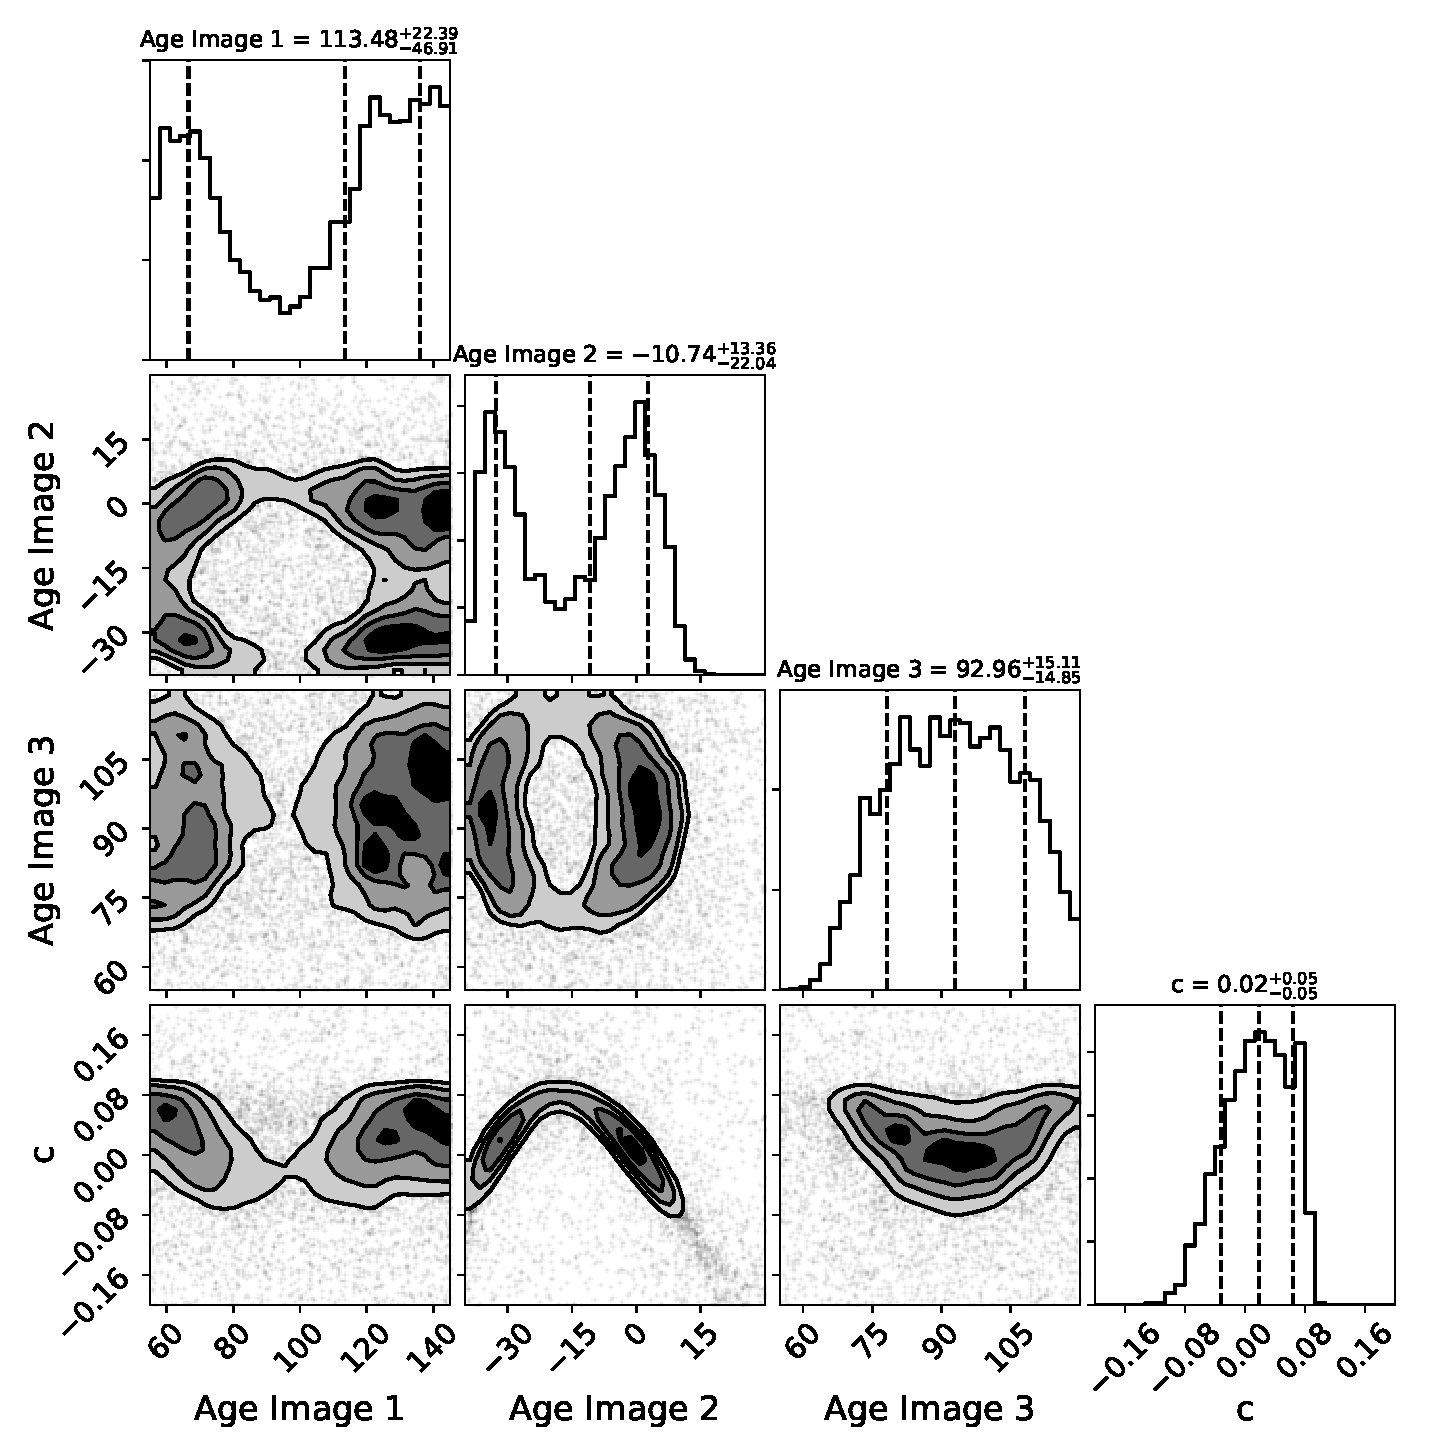
\includegraphics[width=0.75\textwidth]{Images/corner_color_curve_fit_with_c_prior.pdf}
    \caption{Corner plot for color curve nested sampling with prior on c.}
    \label{fig:corner_cfit}
\end{figure*}
\begin{figure*}
    \centering
    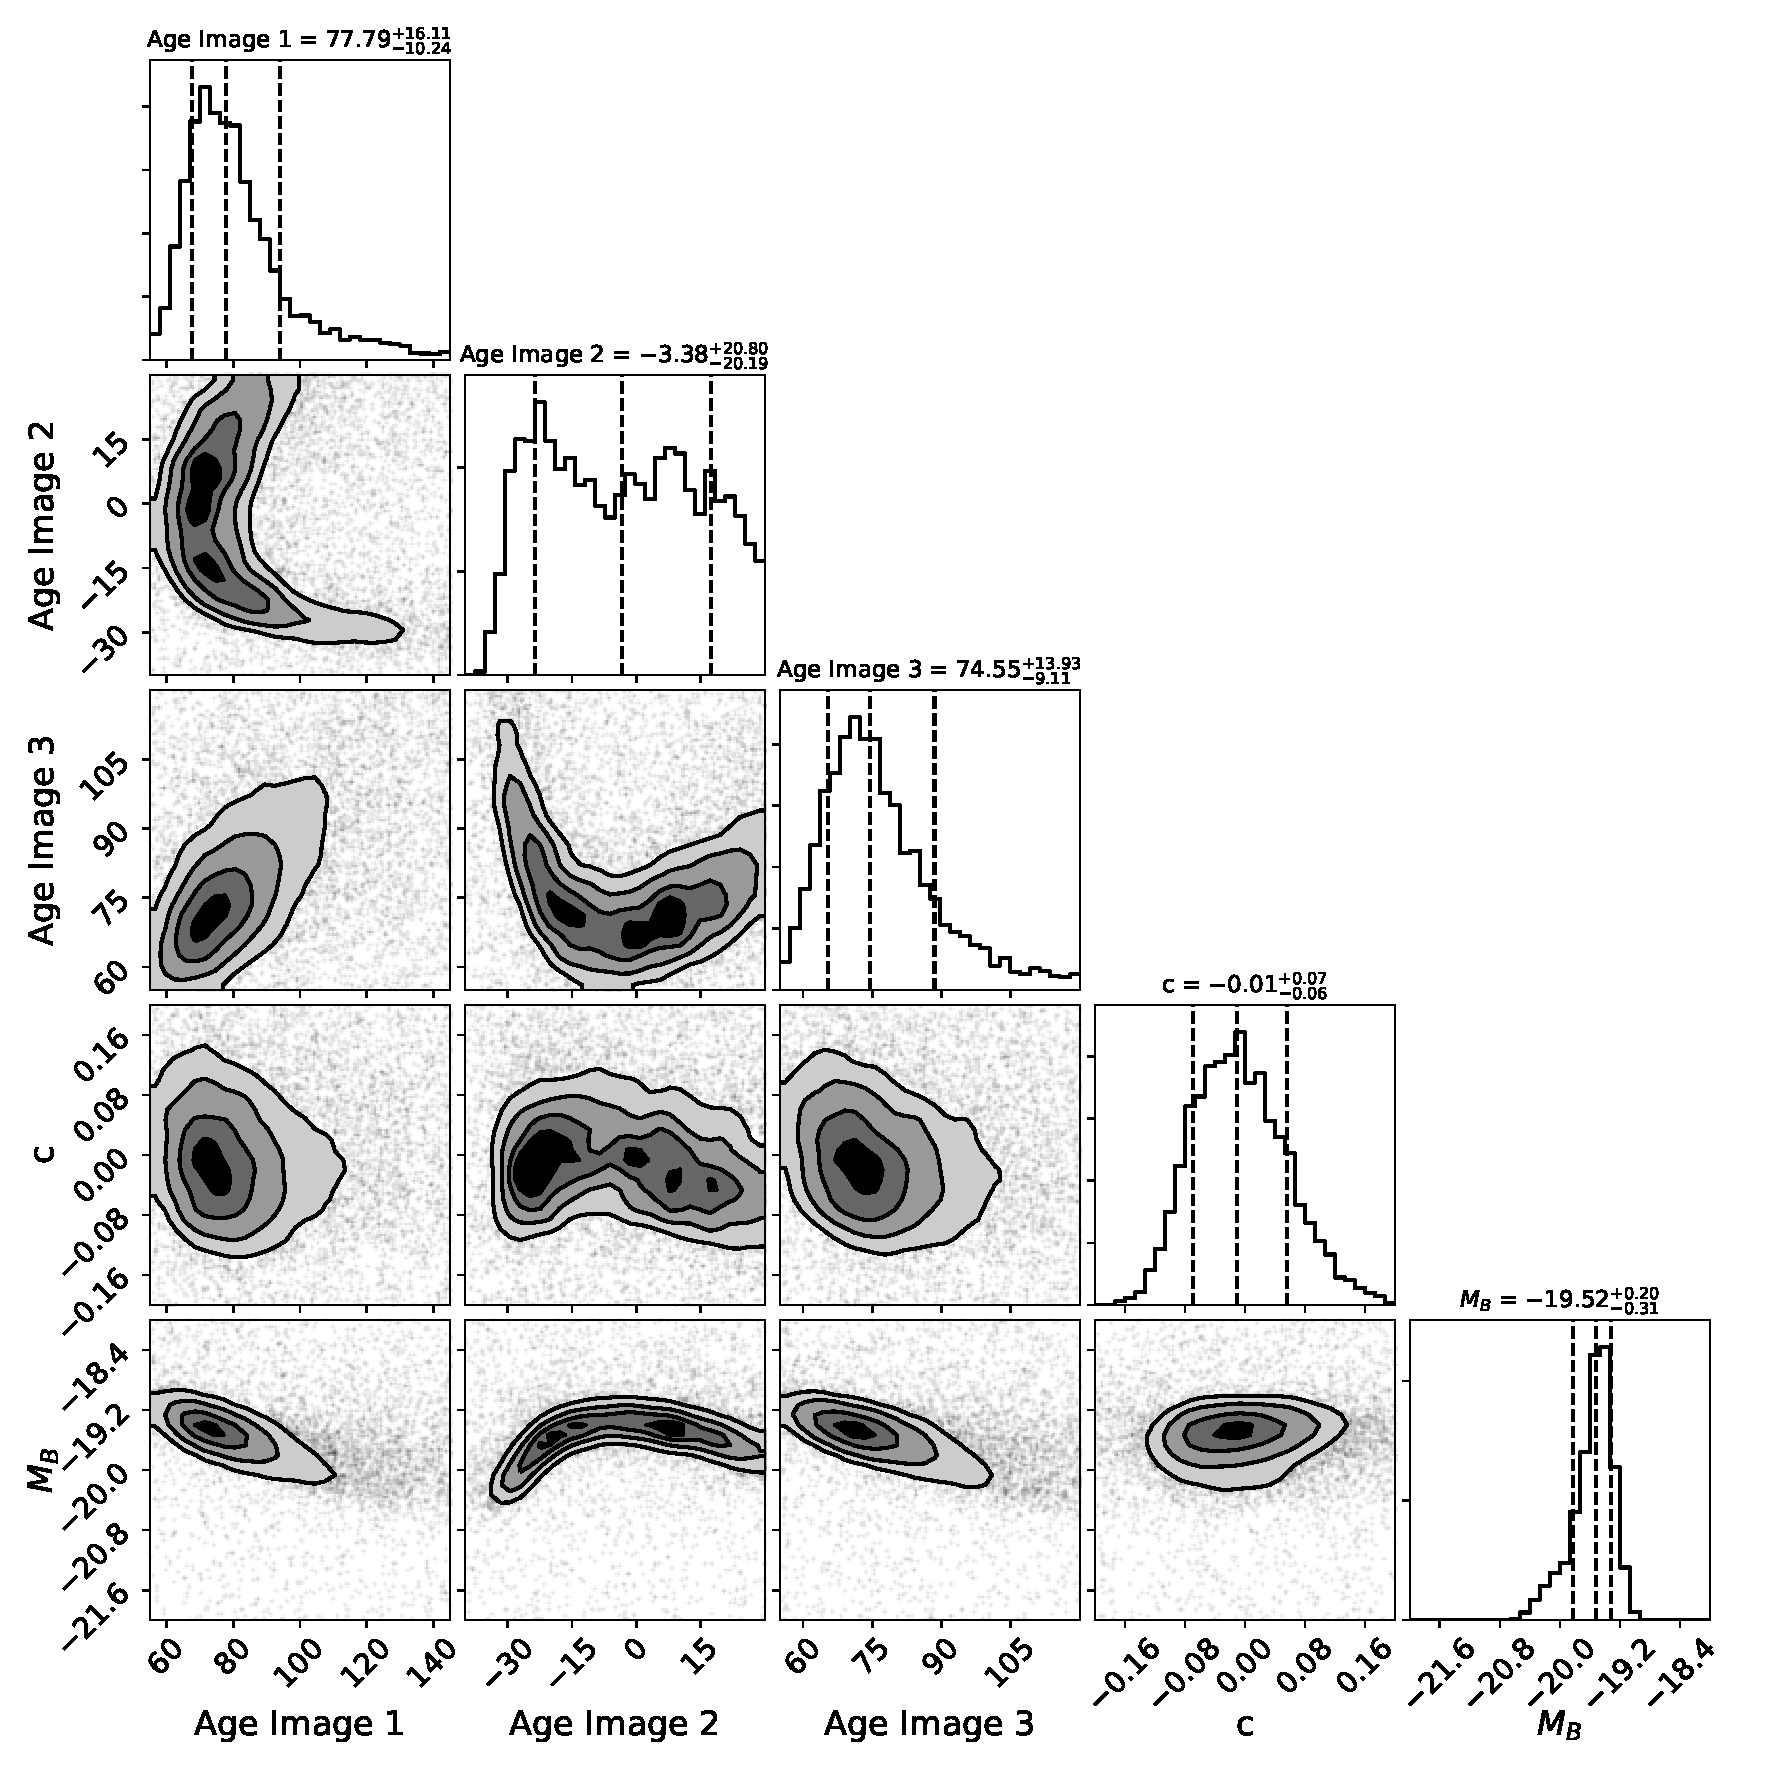
\includegraphics[width=0.75\textwidth]{Images/corner_model_E.pdf}
    \caption{Corner plot for light curve nested sampling using model E.}
    \label{fig:corner_modelE}
\end{figure*}
\begin{figure*}
    \centering
    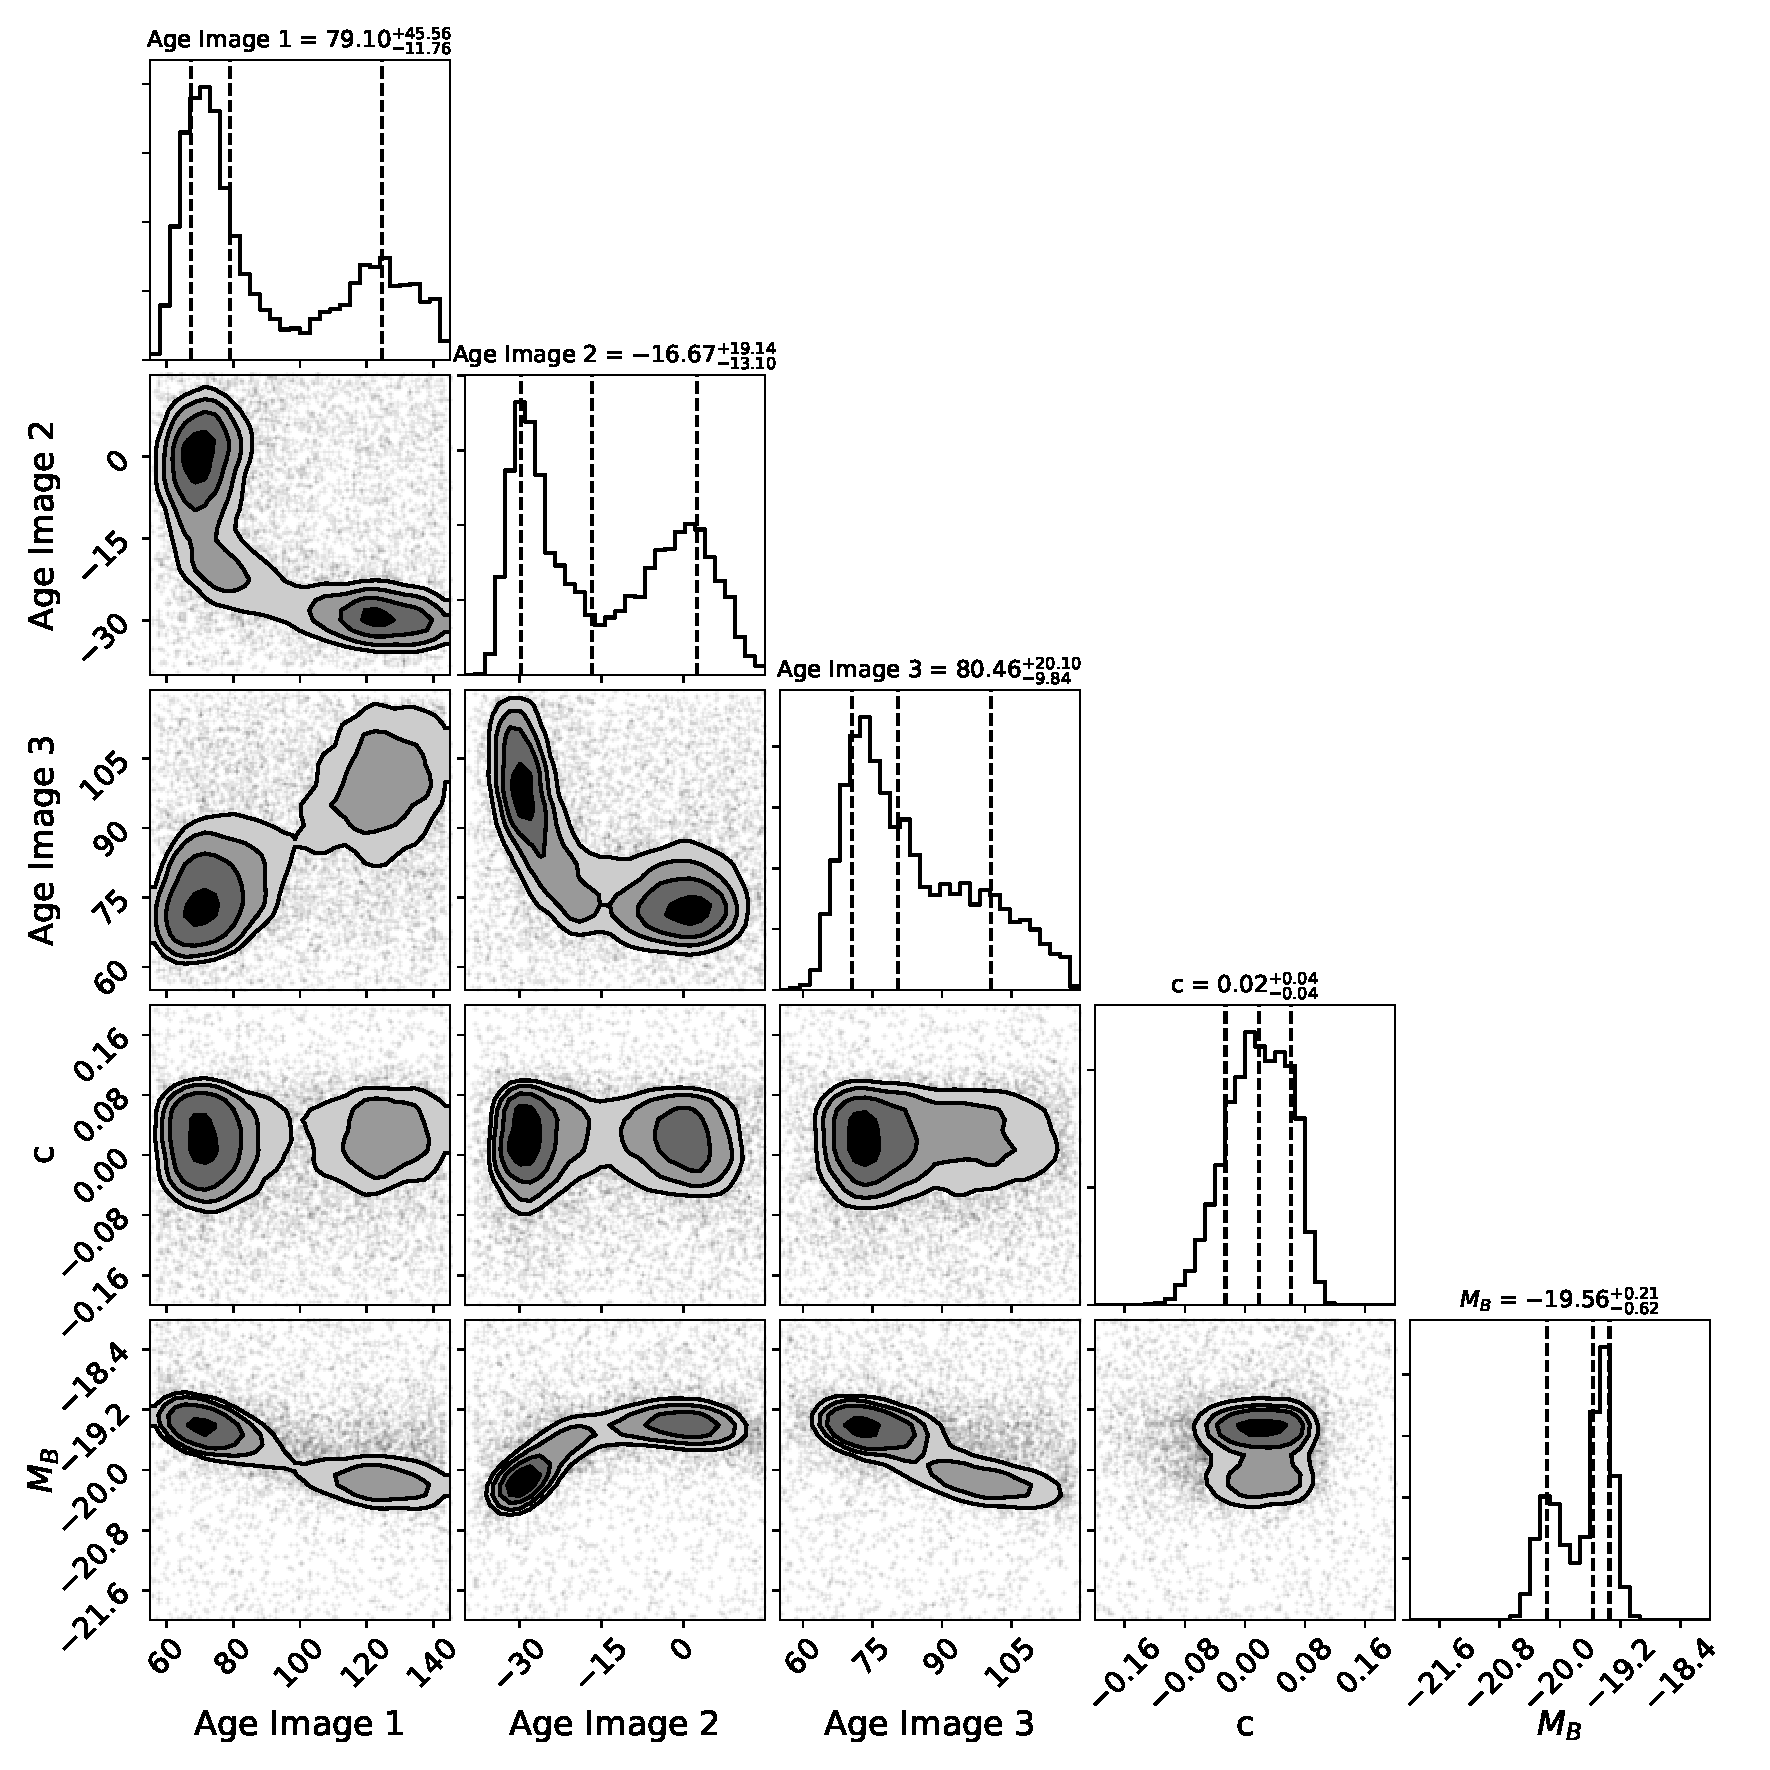
\includegraphics[width=0.75\textwidth]{Images/corner_combined_lc_color_model_E.pdf}
    \caption{Corner plot for combined color curve and model E light curve nested sampling.}
    \label{fig:corner_combined}
\end{figure*}



\end{document}
